%%%%%%%%%%%%%%%%%%%%%%%%%%%%%%%%%%%%%%%%%%%%%%%%%%%%%%%%%%%%%%%%%%%%%%%%%
%  Zawartość: Główny plik szablonu pracy dyplomowej (inżynierskiej).
%  Opracował: Tomasz Kubik <tomasz.kubik@pwr.edu.pl>
%  Data: kwiecień 2016
%  Wersja: 0.2
%%%%%%%%%%%%%%%%%%%%%%%%%%%%%%%%%%%%%%%%%%%%%%%%%%%%%%%%%%%%%%%%%%%%%%%%%

\documentclass[a4paper,onecolumn,oneside,12pt,extrafontsizes]{memoir}
% W celu przygotowania wydruku do archiwum należy przesłonić komendę powyższą
% dwoma poniższymi komendami:
%\documentclass[a4paper,onecolumn,twoside,10pt]{memoir} 
%\renewcommand{\normalsize}{\fontsize{8pt}{10pt}\selectfont}

%\usepackage[cp1250]{inputenc} % jeśli kodowanie edytowanych plików to cp1250 
\usepackage[utf8]{inputenc} % jeśli kodowanie edytowanych plików to UTF8
\usepackage[T1]{fontenc}
\usepackage[polish]{babel}
%\DisemulatePackage{setspace}
\usepackage{setspace}
\usepackage{tabularx}
\usepackage{color,calc}
%\usepackage{soul} % pakiet z komendami do podkreślania tekstu

\usepackage{ebgaramond} % pakiet z czcionkami garamond, potrzebny tylko do strony tytułowej, musi wystąpić przed pakietem tgtermes

%% Aby uzyskać polskie literki w pdfie (a nie zlepki) korzystamy z pakietu czcionek tgterms. 
%% W pakiecie tym są zdefiniowane klony czcionek Times o kształtach: normalny, pogrubiony, italic, italic pogrubiony.
%% W pakiecie tym brakuje czcionki o kształcie: slanted (podobny do italic). 
%% Jeśli w dokumencie gdzieś zostanie zastosowana czcionka slanted (np. po użyciu komendy \textsl{}), to
%% latex dokona podstawienia na czcionkę standardową i zgłosi to w ostrzeżeniu (warningu).
%% Ponadto tgtermes to czcionka do tekstu. Wszelkie matematyczne wzory będą sformatowane domyślną czcionką do wzorów.
%% Jeśli wzory mają być sformatowane z wykorzystaniem innych czcionek, trzeba to jawnie zadeklarować.

%% Po zainstalowaniu pakietu tgtermes może będzie trzeba zauktualizować informacje 
%% o dostępnych fontach oraz mapy. Można to zrobić z konsoli (jako administrator)
%% initexmf --admin --update-fndb
%% initexmf --admin --mkmaps

\usepackage{tgtermes}   
\renewcommand*\ttdefault{txtt}

% We wcześniejszej wersji szablonu korzystano z innych czcionek. Dla celów historycznych pozostawiono je w komentarzu
%\usepackage{mathptmx} % pakiet będący następcą pakietów times and mathptm, niestety polskie literki są zlepkami
%\usepackage{newtxtext,newtxmath} % pakiety dostarczające Times dla tekstów i wzorów matematycznych,  
%                                  rozwiązuje problemy występujące w mathptmx, ale wymaga zainstalowania
%                                  dodatkowych pakietów oraz uruchomienia updmap (konsola administratora)
%                                  niestety polskie literki są zlepkami
%\usepackage{newtxmath,tgtermes} % można też połączyć czcionki do tekstu i czcionki do wzorów

\usepackage{listings} % pakiet do prezentacji kodu. 
%Wcześniej był problem z polskimi znakami w otoczeniu lstlisting, stąd pozostawiono w komentarzu zastosowane wtedy rozwiązanie: 
\lstset{literate=%-
{ą}{{\k{a}}}1 {ć}{{\'c}}1 {ę}{{\k{e}}}1 {ł}{{\l{}}}1 {ń}{{\'n}}1 {ó}{{\'o}}1 {ś}{{\'s}}1 {ż}{{\.z}}1 {ź}{{\'z}}1 {Ą}{{\k{A}}}1 {Ć}{{\'C}}1 {Ę}{{\k{E}}}1 {Ł}{{\L{}}}1 {Ń}{{\'N}}1 {Ó}{{\'O}}1 {Ś}{{\'S}}1 {Ż}{{\.Z}}1 {Ź}{{\'Z}}1 }%{\ \ }{{\ }}1}

% Choć możliwe jest zastosowanie różnych pakietów formatujących tabele, zaleca się tego nie robić.
%\usepackage{longtable}
%\usepackage{ltxtable}
%\usepackage{tabulary}

%%%%%%%%%%%%%%%%%%%%%%%%%%%%%%%%%%%%%%%%%%%%%%%%%%%
%% Ustawienia odpowiedzialne za sposób łamania dokumentu
%% i ułożenie elementów pływających
%%%%%%%%%%%%%%%%%%%%%%%%%%%%%%%%%%%%%%%%%%%%%%%%%%%
%\hyphenpenalty=10000		% nie dziel wyrazów zbyt często
\clubpenalty=10000      %kara za sierotki
\widowpenalty=10000  % nie pozostawiaj wdów
\brokenpenalty=10000		% nie dziel wyrazów między stronami
\exhyphenpenalty=999999		% nie dziel słów z myślnikiem
\righthyphenmin=3			% dziel minimum 3 litery

%\tolerance=4500
%\pretolerance=250
%\hfuzz=1.5pt
%\hbadness=1450

\renewcommand{\topfraction}{0.95}
\renewcommand{\bottomfraction}{0.95}
\renewcommand{\textfraction}{0.05}
\renewcommand{\floatpagefraction}{0.35}

%%%%%%%%%%%%%%%%%%%%%%%%%%%%%%%%%%%%%%%%%%%%%%%%%%%
%%  Ustawienia rozmiarów: tekstu, nagłówka i stopki, marginesów
%%  dla dokumentów klasy memoir 
%%%%%%%%%%%%%%%%%%%%%%%%%%%%%%%%%%%%%%%%%%%%%%%%%%%
\setlength{\headsep}{10pt} 
\setlength{\headheight}{13.6pt} % wartość baselineskip dla czcionki 11pt tj. \small wynosi 13.6pt
\setlength{\footskip}{\headsep+\headheight}
\setlength{\uppermargin}{\headheight+\headsep+1cm}
\setlength{\textheight}{\paperheight-\uppermargin-\footskip-1.5cm}
\setlength{\textwidth}{\paperwidth-5cm}
\setlength{\spinemargin}{2.5cm}
\setlength{\foremargin}{2.5cm}
\setlength{\marginparsep}{2mm}
\setlength{\marginparwidth}{2.3mm}
%\settrimmedsize{297mm}{210mm}{*}
%\settrims{0mm}{0mm}	
\checkandfixthelayout[fixed] % konieczne, aby się dobrze wszystko poustawiało
%%%%%%%%%%%%%%%%%%%%%%%%%%%%%%%%%%%%%%%%%%%%%%%%
%%  Ustawienia odległości linii, wcięć, odstępów
%%%%%%%%%%%%%%%%%%%%%%%%%%%%%%%%%%%%%%%%%%%%%%%%
\linespread{1}
%\linespread{1.241}
\setlength{\parindent}{14.5pt}
%\setbeforesecskip{10pt plus 0.5ex}%{-3.5ex \@plus -1ex \@minus -.2ex}
%\setaftersecskip{10pt plus 0.5ex}%\onelineskip}
%\setbeforesubsecskip{8pt plus 0.5ex}%{-3.5ex \@plus -1ex \@minus -.2ex}
%\setaftersubsecskip{8pt plus 0.5ex}%\onelineskip}
%\setlength\floatsep{6pt plus 2pt minus 2pt} 
%\setlength\intextsep{12pt plus 2pt minus 2pt} 
%\setlength\textfloatsep{12pt plus 2pt minus 2pt} 

%%%%%%%%%%%%%%%%%%%%%%%%%%%%%%%%%%%%%%%%%%%%%%%%%%%
%%  Pakiety i komendy zastosowane tylko do zamieszczenia informacji o użytych komendach i fontach
%%  Normalnie nie są potrzebne, można je zamarkować podczas redakcji pracy
%%%%%%%%%%%%%%%%%%%%%%%%%%%%%%%%%%%%%%%%%%%%%%%%%%%
\usepackage{memlays}     % extra layout diagrams, zastosowane w szblonie do 'debuggowania', używa pakietu layouts
%\usepackage{layouts}
\usepackage{printlen} % pakiet do wyświetlania wartości zdefiniowanych długości, stosowany do 'debuggowania'
\uselengthunit{pt}
\makeatletter
\newcommand{\showFontSize}{\f@size pt} % makro wypisujące wielkość bieżącej czcionki
\makeatother
% do pokazania ramek można byłoby użyć:
%\usepackage{showframe} 


%%%%%%%%%%%%%%%%%%%%%%%%%%%%%%%%%%%%%%%%%%%%%%%%%%%
%%  Formatowanie list wyliczeniowych, wypunktowań i własnych otoczeń
%%%%%%%%%%%%%%%%%%%%%%%%%%%%%%%%%%%%%%%%%%%%%%%%%%%

% Domyślnie wypunktowania mają zadeklatorowane znaki, które nie występują w tgtermes
% Aby latex nie podstawiał w ich miejsca znaków z czcionki standardowej można zrobić podstawienie:
%    \DeclareTextCommandDefault{\textbullet}{\ensuremath{\bullet}}
%    \DeclareTextCommandDefault{\textasteriskcentered}{\ensuremath{\ast}}
%    \DeclareTextCommandDefault{\textperiodcentered}{\ensuremath{\cdot}}
% Jednak jeszcze lepszym pomysłem jest zdefiniowanie otoczeń z wykorzystaniem enumitem
\usepackage{enumitem} % pakiet pozwalający zarządzać formatowaniem list wyliczeniowych
\setlist{noitemsep,topsep=4pt,parsep=0pt,partopsep=4pt,leftmargin=*} % zadeklarowane parametry pozwalają uzyskać 'zwartą' postać wypunktowania bądź wyliczenia
\setenumerate{labelindent=0pt,itemindent=0pt,leftmargin=!,label=\arabic*.} % można zmienić \arabic na \alph, jeśli wyliczenia mają być z literkami
\setlistdepth{4} % definiujemy głębokość zagnieżdżenia list wyliczeniowych do 4 poziomów
\setlist[itemize,1]{label=$\bullet$}  % definiujemy, jaki symbol ma być użyty w wyliczeniu na danym poziomie
\setlist[itemize,2]{label=\normalfont\bfseries\textendash}
\setlist[itemize,3]{label=$\ast$}
\setlist[itemize,4]{label=$\cdot$}
\renewlist{itemize}{itemize}{4}

%%%http://tex.stackexchange.com/questions/29322/how-to-make-enumerate-items-align-at-left-margin
%\renewenvironment{enumerate}
%{
%\begin{list}{\arabic{enumi}.}
%{
%\usecounter{enumi}
%%\setlength{\itemindent}{0pt}
%%\setlength{\leftmargin}{1.8em}%{2zw} % 
%%\setlength{\rightmargin}{0zw} %
%%\setlength{\labelsep}{1zw} %
%%\setlength{\labelwidth}{3zw} % 
%\setlength{\topsep}{6pt}%
%\setlength{\partopsep}{0pt}%
%\setlength{\parskip}{0pt}%
%\setlength{\parsep}{0em} % 
%\setlength{\itemsep}{0em} % 
%%\setlength{\listparindent}{1zw} % 
%}
%}{
%\end{list}
%}

\makeatletter
\renewenvironment{quote}{
	\begin{list}{}
	{
	\setlength{\leftmargin}{1em}
	\setlength{\topsep}{0pt}%
	\setlength{\partopsep}{0pt}%
	\setlength{\parskip}{0pt}%
	\setlength{\parsep}{0pt}%
	\setlength{\itemsep}{0pt}
	}
	}{
	\end{list}}
\makeatother

%%%%%%%%%%%%%%%%%%%%%%%%%%%%%%%%%%%%%%%%%
%%  Pakiet do generowania indeksu (ważne, aby wstawić przed hyperref)
%%%%%%%%%%%%%%%%%%%%%%%%%%%%%%%%%%%%%%%%%
\DisemulatePackage{imakeidx}
\usepackage[makeindex,noautomatic]{imakeidx} % tutaj mówimy, żeby indeks nie generował się automatycznie, 

%\usepackage[noautomatic]{imakeidx} 
\makeindex

\makeatletter
%%%\renewenvironment{theindex}
							 %%%{\vskip 10pt\@makeschapterhead{\indexname}\vskip -3pt%
								%%%\@mkboth{\MakeUppercase\indexname}%
												%%%{\MakeUppercase\indexname}%
								%%%\vspace{-3.2mm}\parindent\z@%
								%%%\renewcommand\subitem{\par\hangindent 16\p@ \hspace*{0\p@}}%%
								%%%\phantomsection%
								%%%\begin{multicols}{2}
								%%%%\thispagestyle{plain}
								%%%\parindent\z@                
								%%%%\parskip\z@ \@plus .3\p@\relax
								%%%\let\item\@idxitem}
							 %%%{\end{multicols}\clearpage}
%%%
\makeatother


\usepackage{ifpdf}
%\newif\ifpdf \ifx\pdfoutput\undefined
%\pdffalse % we are not running PDFLaTeX
%\else
%\pdfoutput=1 % we are running PDFLaTeX
%\pdftrue \fi
\ifpdf
 \usepackage[pdftex,bookmarks,breaklinks,unicode]{hyperref}
 \usepackage[pdftex]{graphicx}
 \DeclareGraphicsExtensions{.pdf,.jpg,.mps,.png}
\pdfcompresslevel=9
\pdfoutput=1
\makeatletter
\AtBeginDocument{
  \hypersetup{
	pdfinfo={
    Title = {\@title},
    Author = {\@author},
    Subject={},
    Keywords={słowa kluczowe},
  }}
}
\makeatother
\else
\usepackage{graphicx}
\DeclareGraphicsExtensions{.eps,.ps,.jpg,.mps,.png}
\fi
\sloppy


%\graphicspath{{rys01/}{rys02/}}


%%%%%%%%%%%%%%%%%%%%%%%%%%%%%%%%%%%%%%%%%
% Metadane dla pdfa


%\ifpdf
%\pdfinfo{
   %/Author (Nicola Talbot)
   %/Title  (Creating a PDF document using PDFLaTeX)
   %/CreationDate (D:20040502195600)
   %/ModDate (D:\pdfdate)
   %/Subject (PDFLaTeX)
   %/Keywords (PDF;LaTeX)
%}
%\fi

% Deklaracja głębokościu numeracji
\setcounter{secnumdepth}{2}
\setcounter{tocdepth}{2}
\setsecnumdepth{subsection} % activating subsubsec numbering in doc


% Kropki po numerach sekcji
\makeatletter
\def\@seccntformat#1{\csname the#1\endcsname.\quad}
\def\numberline#1{\hb@xt@\@tempdima{#1\if&#1&\else.\fi\hfil}}
\makeatother

\renewcommand{\chapternumberline}[1]{#1.\quad}
\renewcommand{\cftchapterdotsep}{\cftdotsep}

%\definecolor{niceblue}{rgb}{.168,.234,.671}

% Czcionka do podpisów tabel i rysunków
\captionnamefont{\small}
\captiontitlefont{\small}
% makro pozwalające zmienić sposób wypisywania rozdziału
%\def\printchaptertitle##1{\fonttitle \space \thechapter.\space ##1} 

%\usepackage{ltcaption}
% The ltcaption package supports \CaptionLabelFont & \CaptionTextFont introduced by the NTG document classes
%\renewcommand\CaptionLabelFont{\small}
%\renewcommand\CaptionTextFont{\small}

% Przedefiniowanie etykiet w podpisach tabel i rysunków
%\AtBeginDocument{% 
        \addto\captionspolish{% 
        \renewcommand{\tablename}{Tab.}% 
}%} 

%\AtBeginDocument{% 
%        \addto\captionspolish{% 
%        \renewcommand{\chaptername}{Rozdział}% 
%}} 

%\AtBeginDocument{% 
        \addto\captionspolish{% 
        \renewcommand{\figurename}{Rys.}% 
}%}


%\AtBeginDocument{% 
        \addto\captionspolish{% 
        \renewcommand{\bibname}{Literatura}% 
}%}

%\AtBeginDocument{% 
        \addto\captionspolish{% 
        \renewcommand{\listfigurename}{Spis rysunków}% 
}%}

%\AtBeginDocument{% 
        \addto\captionspolish{% 
        \renewcommand{\listtablename}{Spis tabel}% 
}%}

%\AtBeginDocument{% 
        \addto\captionspolish

%%%%%%%%%%%%%%%%%%%%%%%%%%%%%%%%%%%%%%%%%%%%%%%%%%%%%%%%%%%%%%%%%%                  
%% Definicje stopek i nagłówków
%%%%%%%%%%%%%%%%%%%%%%%%%%%%%%%%%%%%%%%%%%%%%%%%%%%%%%%%%%%%%%%%%%                  
\addtopsmarks{headings}{%
\nouppercaseheads % added at the beginning
}{%
\createmark{chapter}{both}{shownumber}{}{. \space}
%\createmark{chapter}{left}{shownumber}{}{. \space}
\createmark{section}{right}{shownumber}{}{. \space}
}%use the new settings

\makeatletter
\copypagestyle{outer}{headings}
\makeoddhead{outer}{}{}{\small\itshape\rightmark}
\makeevenhead{outer}{\small\itshape\leftmark}{}{}
\makeoddfoot{outer}{\small\@author:~\@titleShort}{}{\small\thepage}
\makeevenfoot{outer}{\small\thepage}{}{\small\@author:~\@title}
\makeheadrule{outer}{\linewidth}{\normalrulethickness}
\makefootrule{outer}{\linewidth}{\normalrulethickness}{2pt}
\makeatother

% fix plain
\copypagestyle{plain}{headings} % overwrite plain with outer
\makeoddhead{plain}{}{}{} % remove right header
\makeevenhead{plain}{}{}{} % remove left header
\makeevenfoot{plain}{}{}{}
\makeoddfoot{plain}{}{}{}

\copypagestyle{empty}{headings} % overwrite plain with outer
\makeoddhead{empty}{}{}{} % remove right header
\makeevenhead{empty}{}{}{} % remove left header
\makeevenfoot{empty}{}{}{}
\makeoddfoot{empty}{}{}{}


%%%%%%%%%%%%%%%%%%%%%%%%%%%%%%%%%%%%%%%
%% Definicja strony tytułowej 
%%%%%%%%%%%%%%%%%%%%%%%%%%%%%%%%%%%%%%%
\makeatletter
%Uczelnia
\newcommand\uczelnia[1]{\renewcommand\@uczelnia{#1}}
\newcommand\@uczelnia{}
%Wydział
\newcommand\wydzial[1]{\renewcommand\@wydzial{#1}}
\newcommand\@wydzial{}
%Kierunek
\newcommand\kierunek[1]{\renewcommand\@kierunek{#1}}
\newcommand\@kierunek{}
%Specjalność
\newcommand\specjalnosc[1]{\renewcommand\@specjalnosc{#1}}
\newcommand\@specjalnosc{}
%Tytuł po angielsku
\newcommand\titleEN[1]{\renewcommand\@titleEN{#1}}
\newcommand\@titleEN{}
%Tytuł krótki
\newcommand\titleShort[1]{\renewcommand\@titleShort{#1}}
\newcommand\@titleShort{}
%Promotor
\newcommand\promotor[1]{\renewcommand\@promotor{#1}}
\newcommand\@promotor{}

%\usepackage[absolute]{textpos} % zamarkowano, bo ostatecznie wykorzystano otoczenie picture

\def\maketitle{%
  \pagestyle{empty}%
%%\garamond 
	\fontfamily{\ebgaramond@family}\selectfont % na stronie tytułowej czcionka garamond
%%%%%%%%%%%%%%%%%%%%%%%%%%%%%%%%%%%%%	
%% Poniżej, w otoczniu picture, wstawiono tytuł i autora. 
%% Tytuł (z autorem) musi znaleźć się w obszarze 
%% odpowiadającym okienku 110mmx75mm, którego lewy górny róg 
%% jest w położeniu 77mm od lewej i 111mm od górnej  krawędzi strony 
%% (tak wynika z wycięcia na okładce). 
%% Poniższy kod musi być użyty dokładnie w miejscu gdzie jest.
%% Jeśli tytuł nie mieści się w okienku, to należy tak pozmieniać 
%% parametry użytych komend, aby ten przydługi tytuł jednak 
%% upakować go do okienka.
%%
%% Sama okładka (kolorowa strona z wycięciem, do pobrania z dydaktyki) 
%% powinna być przycięta o 3mm od każdej z krawędzi.
%% Te 3mm pewnie zostawiono na ewentualne spady czy też specjalną oprawę.
%%%%%%%%%%%%%%%%%%%%%%%%%%%%%%%%%%%%%	
\newlength{\tmpfboxrule}
\setlength{\tmpfboxrule}{\fboxrule}
\setlength{\fboxsep}{2mm}
\setlength{\fboxrule}{0mm} 
%\setlength{\fboxrule}{0.1mm} %% jeśli chcemy zobaczyć ramkę
\setlength{\unitlength}{1mm}
\begin{picture}(0,0)
\put(26,-124){\fbox{
\parbox[c][71mm][c]{104mm}{\centering%\lineskip=34pt 
\fontsize{16pt}{18pt}\selectfont \@title\\[5mm]
\fontsize{16pt}{18pt}\selectfont \@titleEN\\[20mm]
\fontsize{16pt}{18pt}\selectfont AUTOR:\\[2mm]
\fontsize{14pt}{16pt}\selectfont \@author}
}
}
\end{picture}
\setlength{\fboxrule}{\tmpfboxrule} 
%%%%%%%%%%%%%%%%%%%%%%%%%%%%%%%%%%%%%
%% Reszta strony z nazwą uczelni, wydziału, kierunkiem, specjalnością
%% promotorem, oceną pracy, miastem i rokiem
	{\centering%\vspace{-1cm}
		{\fontsize{22pt}{24pt}\selectfont \@uczelnia}\\[0.4cm]
		{\fontsize{22pt}{24pt}\selectfont \@wydzial}\\[0.5cm]
		  \hrule %\vspace*{0.7cm}
	}
{\flushleft\fontsize{14pt}{16pt}\selectfont%
\begin{tabular}{ll}
KIERUNEK: & \@kierunek\\
SPECJALNOŚĆ: & \@specjalnosc\\
\end{tabular}\\[1.3cm]
}
{\centering
{\fontsize{32pt}{36pt}\selectfont PRACA DYPLOMOWA}\\[0.5cm]
{\fontsize{32pt}{36pt}\selectfont INŻYNIERSKA}\\[2.5cm]
}
\vfill
\begin{tabularx}{\linewidth}{p{6cm}l}
		&{\fontsize{16pt}{18pt}\selectfont PROWADZĄCY PRACĘ:}\\[2mm] %UWAGA: tutaj jest miejsce na nazwisko promotora pracy
		&{\fontsize{14pt}{16pt}\selectfont \@promotor}\\[10mm]
		&{\fontsize{16pt}{18pt}\selectfont OCENA PRACY:}\\[20mm]
	\end{tabularx}
\vspace{2cm}
\hrule\vspace*{0.3cm}
{\centering
{\fontsize{16pt}{18pt}\selectfont \@date}\\[0cm]
}
%\ungaramond
\normalfont
 \cleardoublepage
}
\makeatother
%%%%%%%%%%%%%%%%%%%%%%%%%%%%%%%%%%%%%%%%%

%\AtBeginDocument{\addtocontents{toc}{\protect\thispagestyle{empty}}}




%%%%%%%%%%%%%%%%%%%%%%%%%%%%%%%%%%%%%%%%%
%%  Metadane dokumentu 
%%%%%%%%%%%%%%%%%%%%%%%%%%%%%%%%%%%%%%%%%
\title{Aplikacja do planowania domowego budżetu}
\titleShort{Aplikacja do planowania domowego budżetu}
\titleEN{Household budget planning application}
\author{Paweł Żółtaniecki}
\uczelnia{POLITECHNIKA WROCŁAWSKA}
\wydzial{WYDZIAŁ ELEKTRONIKI}
\kierunek{INFORMATYKA}
\specjalnosc{INŻYNIERIA SYSTEMÓW INFORMATYCZNYCH}
\promotor{dr inż. Tomasz Kubik, Katedra Informatyki Technicznej}
\date{WROCŁAW, 2019}

% Ustawienie odstępu od góry w nienumerowanych rozdziałach oraz wykazach:
% Spis treści, Spis tabel, Spis rysunków, Indeks rzeczowy

%\newlength{\linespace}
%\setlength{\linespace}{-\beforechapskip-\topskip+\headheight+\topsep}
%\makechapterstyle{noNumbered}{%
%\renewcommand\chapterheadstart{\vspace*{\linespace}}
%}

%% powyższa komenda załatwia to, co robią komendy poniższe dla spisów
%\renewcommand*{\tocheadstart}{\vspace*{\linespace}}
%\renewcommand*{\lotheadstart}{\vspace*{\linespace}}
%\renewcommand*{\lofheadstart}{\vspace*{\linespace}}

%%%%%%%%%%%%%%%%%%%%%%%%%%%%%%%%%%%%%%%%%
%                  Początek dokumentu 
%%%%%%%%%%%%%%%%%%%%%%%%%%%%%%%%%%%%%%%%%
\includeonly{rozdzial01} % jeśli chcemy kompilować tylko fragmenty, to można tu je wpisać

\begin{document}
% Tutaj można przełączyć odstęp między liniami
%\SingleSpacing
%\OnehalfSpacing
%\DoubleSpacing

%\settypeoutlayoutunit{cm} % do debugowania
%\typeoutstandardlayout    % wypisuje na stdout informacje o ustawieniach
\maketitle

\newpage
\thispagestyle{empty}
\mbox{}\vfill
\noindent\begin{tabular}{@{}ll} Opracował: & Tomasz Kubik <tomasz.kubik@pwr.edu.pl>\\
 Data: & maj 2016 
 \end{tabular}\\[15mm]
\noindent
\includegraphics[width=3cm]{by-nc-sa}\newline
{\normalfont 
Szablon jest udostępniany na licencji Creative Commons: \emph{Uznanie autorstwa -- Użycie niekomercyjne -- Na tych samych warunkach, 3.0 Polska}, Wrocław 2016. \\[2pt]
Oznacza to, że wszystkie zawarte  nim treści można kopiować i  wykorzystywać do celów niekomercyjnych, a także tworzyć na ich podstawie utwory zależne pod warunkiem podania autora i~nazwy licencjodawcy oraz udzielania na utwory zależne takiej samej licencji. Tekst licencji jest dostępny pod adresem: \url{http://creativecommons.org/licenses/by-nc-sa/3.0/pl/}.}
\newpage


\chapterstyle{noNumbered}
\pagestyle{outer}
\mbox{}\pdfbookmark[0]{Spis treści}{spisTresci.1}
\tableofcontents* 

\newpage
\mbox{}\pdfbookmark[0]{Spis rysunków}{spisRysunkow.1}
%\addcontentsline{toc}{chapter}{Spis rysunków}
\listoffigures*
\begin{flushleft}

\end{flushleft}
%{%
%\let\oldnumberline\numberline%
%\renewcommand{\numberline}{\figurename~\oldnumberline}%
%\listoffigures%
%}


\newpage
\mbox{}\pdfbookmark[0]{Spis tabel}{spisTabel.1}
%\addcontentsline{toc}{chapter}{Spis tabel}
\listoftables*

\chapter*{Skróty}\mbox{}\pdfbookmark[0]{Skróty}{skroty.1}
\label{sec:skroty}
\noindent
\begin{description}
  \item [QR] (ang.\ \emph{quick response})
  \item [API] (ang.\ \emph{Application Programming Interface})
  \item [URL] (ang.\ \emph{Uniform Resource Locator})
  \item [ISO] (ang.\ \emph{International Organization for Standardization})
  \item [OData] (ang.\ \emph{Open Data Protocol})
  \item [HTTP] (ang.\ \emph{Hypertext Transfer Protoco})
  \item [JSON] (ang. \ \emph{JavaScript Object Notation})
  \item [HATEOAS] (ang. \ \emph{Hypermedia As Transfer Engine Of Application State})
  %\item [OData] (ang.\ \emph{Open Data Protocol})
\end{description}
 %skróty można sobie pominąć
\chapterstyle{default}
\chapter{Wstęp}
\label{chap:wstep}
\section{Wprowadzenie}
\label{sec:wprowadzenie}
Zarządzanie finansami to jeden z ważniejszych aspektów funkcjonowania każdego przedsiębiorstwa, bez względu na rodzaj prowadzonej działalności, a także liczbę pracowników. Rozliczanie przychodów i wydatków jest nie tylko bardzo często obowiązkiem, ale również pomocą w panowaniu nad przepływem środków finansowych. 

Jako szczególny typ przedsiębiorstwa można uznać gospodarstwo domowe, czyli po prostu rodzinę. Z ekonomicznego punktu widzenia jej celem jest zaspokajanie wspólnych i osobistych potrzeb. Rodzina jest też zespołem osób, które wspólnie podejmują decyzję o swoim podstawowym utrzymaniu i zarządzaniu wniesionymi do budżetu domowego środkami. Gospodarstwem domowym można także nazwać pojedynczą osobę utrzymującą się samodzielnie~\cite{gospodarstwo-domowe}.

W dobie rosnącej konsumpcji oraz na skutek celowego stosowania różnych technik pobudzania zapotrzebowania przez producentów panowanie nad wydatkami zaczyna sprawiać sporo trudności. Problemem staje się odróżnienie zachcianek od tego, co z punktu widzenia funkcjonowania rodziny jest niezbędne. W konsekwencji dość łatwo jest doprowadzić do załamania całego domowego budżetu.

Z panowaniem nad wydatkami bezpośrednio wiąże się monitorowanie dochodów i~inwestycji gospodarstwa domowego. Oprócz tradycyjnych dochodów z tytułu etatu, rodzina może mieć inne źródła przychodu, jak na przykład praca dorywcza czy wynajem nieruchomości. Nieruchomości to niejedyna możliwość ulokowania oszczędności gospodarstwa domowego. Innymi przykładami inwestycji mogą być lokaty, obligacje skarbowe, złoto, a nawet akcje giełdowe. Coraz częściej jednym ze sposobów ich zaoszczędzenia jest dołączanie do programów lojalnościowych, które wiążą się dodatkowymi rabatami oraz bonami na zakupy. Nierzadko też bogata oferta banków pozwala na odłożenie dodatkowej gotówki czy zbieranie punktów w podobnych programach. W~obu przypadkach warunkiem uczestnictwa w promocji jest wyrobienie dodatkowej karty bądź pobranie i rejestracja w aplikacji mobilnej banku lub sprzedawcy.

Kolejnym ważnym aspektem domowych finansów jest trwałość zakupionych towarów, takich, jak na przykład ubrania oraz sprzęt RTV i AGD. Rozklejające się po kilku miesiącach buty, psująca się lodówka, jak również innego rodzaju uszkodzenia i usterki, mogą prowadzić do nadwyrężenia budżetu domowego. Dlatego w wielu domach trzyma się paragony i faktury w celu dokonania potencjalnej reklamacji. Spotykane są rozwiązania umożliwiające zarówno powiązania zakupów z kontem w aplikacji lojalnościowej, jak i dedykowane programy do trzymania dokumentów sprzedażowych w formie elektronicznej.

% TO DO: proszę dołożyć cytowania (do stron domowych wymienonych niżej aplikacji).
Popularną aplikacją, która pozwala na elektroniczne przechowywanie paragonów jest ,,Pan Paragon''. Umożliwia on nie tylko na trzymanie dokumentów sprzedażowych w pamięci lokalnej telefonu, ale również na ich archiwizację w chmurze. Pozwala on także na przechowywanie kart lojalnościowych. Niestety, nie daje możliwości do zarządzania wydatkami i planowania budżetu. Jest też aplikacją dedykowaną jednostce, a nie rodzinie.

Istnieje też wiele programów do zarządzania budżetem domowym. Jednym z przykładów jest ,,Wallet - przychody i wydatki, karty lojalnościowe''. Niestety, zakres oferowanych w nim funkcji jest ograniczony. Użytkownik w darmowej wersji może zdefiniować tylko trzy konta. Nie ma też możliwości integrowania wydatków innych członków rodziny, co komplikuje sprawny nadzór nad całym domowym budżetem.

W ostatnim czasie również supermarkety czy sklepy odzieżowe wypuszczają własne oprogramowanie, umożliwiające branie udziału w programach lojalnościowych. Jednym z nich jest Lidl, którego rozwiązanie oferuje też zapisanie paragonu w aplikacji. Cały proces odbywa się poprzez zeskanowanie kodu QR (ang.~\emph{quick response}) w telefonie. W przypadku tego typu programów, problemem staje się mnogość rozwiązań dla pojedynczych sieci i marek.

Jak widać dbanie o budżet gospodarstwa domowego nie jest rzeczą trywialną. Wielowymiarowość tego zadania może przyprawić osobę odpowiedzialną o zawrót głowy. Dużym utrudnieniem jest brak możliwości synchronizowania działań całej rodziny w ramach jednego systemu. Ponadto nie wystarczy tylko panować nad przychodami i wydatkami. Trzeba wziąć pod uwagę czynniki, takie jak zabezpieczenie się przed utratą środków z powodu przedwczesnego zużycia się produktów, a także  programy lojalnościowe, które oferują atrakcyjne promocje. Tutaj sprawę komplikuje ilość potencjalnych kart i możliwość współdzielenia ich między członkami rodziny. 

W tej pracy dyplomowej zdecydowano się przedstawić projekt aplikacji budżetu domowego, która łączyć będzie wszystkie wyżej wymienione funkcje. Aplikacja ma stać się uniwersalnym narzędziem do zarządzania finansami całej rodziny, ze szczególnym uwzględnieniem roli rodziców i dzieci. Ważnymi funkcjami projektu mają być również te związane z tworzeniem kopii zapasowej paragonów, a także zarządzaniem gwarancjami i mnogością kart lojalnościowych.

\section{Cel i zakres pracy}
\label{sec:cel-zakres}
\subsection{Cel}
\label{subsec:cel}
Celem pracy jest stworzenie aplikacji do zarządzania budżetem domowym, oferującej użytkownikowi bezpieczne i płynne korzystanie z dostarczanych w niej funkcji.
Aplikacja ta w założeniach ma być produktem MVP (ang.~\emph{minimum valuable product}), czyli rozwiązaniem zapewniającym minimalną wartość użytkową.  

Z realizacją celu wiąże się opracowanie koncepcji uniwersalnej aplikacji dla domowego budżetu, która łączyłaby w sobie funkcje innych programów tego typu z~funkcjami programów przechowujących kopie paragonów, a także oferujących możliwość przechowywania kart lojalnościowych, bonów i gwarancji. 
Ponadto w pracy mają powstać założenia projektu elastycznego systemu o nowoczesnej architekturze, umożliwiającej łatwe dodawanie nowych funkcji i integrację z zewnętrznymi dostawcami usług. 

\subsection{Zakres}
\label{subsec:zakres}
W ramach pracy zbudowane zostaną dwie aplikacje webowe. Pierwsza z nich ma oferować graficzny interfejs użytkownika (ang.~\emph{graphical user interface}, GUI) wyświetlany w oknie przeglądarki internetowej, druga zaś ma dostarczyć interfejs programistyczny aplikacji (ang.~\emph{application programming interface}, API)

Zaimplementowane funkcje powinny umożliwiać tworzenie i zarządzania  rachunkiem, tudzież kontem pieniężnym, wraz z możliwością tworzenia wydatków i przychodów. Dodatkowo obsługiwane mają być: tworzenie i przypisywanie kategorii operacji pieniężnych, jak również bezpieczny i nowoczesny sposób rejestracji oraz logowania się użytkownika w systemie, zaimplementowany z wykorzystaniem mechanizmu tokenów.

Aplikacja zostanie dostarczona na środowisko produkcyjne stworzone na platformie Azure. Zostanie ona przetestowana w środowisku deweloperskim oraz produkcyjnym. Ponadto zostanie spisana dokumentacja API.

\section{Układ pracy}
\label{sec:uklad-pracy}
W rozdziale~\ref{chap:wstep} przedstawiono współczesne problemy związane z prowadzeniem domowych finansów i uzasadnienie konieczności stworzenia aplikacji budżetu domowego. Omówiono w~nim również cel pracy inżynierskiej oraz zakres wykonanych prac.

W rozdziale \ref{chap:zalozenia-projektowe} przedstawiono założenia projektowe wraz z~zarysem architektury systemu i~poszczególnych jego komponentów. Zawarto w nim także wymagania funkcjonalne i niefunkcjonalne aplikacji.

Rozdział~\ref{chap:know-how} poświęcono na wstęp teoretyczny. Opisano w nim bazę wiedzy zgromadzoną przez autora podczas przygotowań do realizacji pracy. W podrozdziale~\ref{sec:projektowanie-api} skupiono uwagę na~dobrych praktykach tworzenia API~oraz przydatnych narzędziach. W podrozdziale~\ref{sec:wzorce} przybliżono wykorzystane w~kodzie wzorce projektowe. W podrozdziale~\ref{sec:autoryzacja} dokonano prezentacji użytego mechanizmu autoryzacji i uwierzytelniania.

Szczegóły implementacji opisano w~rozdziale~\ref{chap:implementacja}. W podrozdziale~\ref{sec:struktura-projektu} przedstawiono fizyczną i logiczną strukturę projektu, a~w podrozdziale~\ref{sec:szczegoly-implementacji} -- detale realizacji aplikacji klienckiej (ang.~\emph{frontend}) oraz API działającego po stronie serwera (ang.~\emph{backend}).

Na omówienie testów API i aplikacji klienckiej poświęcono rozdział~\ref{chap:testy}. 

W ostatnim rozdziale~\ref{chap:podsumowanie} zamieszczono podsumowanie pracy wraz z uwagami odnośnie zdobytych doświadczeń.
\chapter{Przygotowania \emph{Know-how}}
\label{chap:know-how}
\section{Projektowanie REST API}
\label{sec:projektowanie-api}
Projektowanie i tworzenie API należy do podstawowych zadań programisty. Poprzez API odbywa się udostępnienie zasobów, jak również z nim związana jest ich ochrona. Zasobami najczęściej są dane, którymi klient może zarządzać w zakresie zdefiniowanym przez przypisane mu uprawnienia. Klientem może być strona internetowa służąca do wyświetlania i zarządzania danymi, a także inna aplikacja serwerowa korzystająca z tych danych.

Użycie API do dostarczania danych do aplikacji klienckiej pozwala rozdzielić logikę widoku po stronie klienta oraz logikę biznesową po stronie serwera. Zaletą tego rozwiązania jest uproszczenie implementacji i w dalszej perspektywie ułatwienie utrzymywania tworzonego programu. Ponadto tak tworzone oprogramowanie jest bardziej elastyczne i łatwiej można je integrować z~innymi systemami. 

Stworzenie dobrego lub zmodyfikowanie już istniejącego API nie jest jednak zadaniem łatwym. Poza tym, że dodawanie funkcji filtrowania, sortowania czy łączenia danych z~różnych zasobów bywa po prostu nużące, to wymusza często konieczność tworzenia nowych punktów dostępu (ang.~\emph{endpoint}) do już istniejących zasobów lub modyfikowania tych już istniejących. Takie działanie niosą ze sobą ryzyko powstawania błędów. Problemem jest także budowanie adresu \texttt{URL} (ang.~\emph{Uniform Resource Locator}). Musi być on elastyczny i intuicyjny, aby można było pracować bez ciągłego wertowania dokumentacji. 

W dalszej części tego rozdziału zebrano zebrano dobre praktyki tworzenia API. Zwrócono też uwagę na zapoczątkowany przez Microsoft i zatwierdzony przez \texttt{ISO} (ang.~\emph{International Organization for Standardization}) protokół \texttt{OData} (ang.~\emph{Open Data Protocol}) i jego gotowe implementacje.

\subsection{Dobre praktyki tworzenia API} 
\label{subsec:api-dobre-praktyki}
Aby stworzyć czytelne i elastyczne REST API należy zastosować się do wielu zasad. Oczywiście nie są one obowiązkowe. Najczęściej jednak stosowanie się do nich ułatwia konsumowanie API i integrowanie go z innymi systemami. Jednym z koniecznych do szybkiej i bezproblemowej pracy z API kroków jest stworzenie i późniejsze aktualizowanie jego dokumentacji. Polecanym i nowoczesnym narzędziem służący do jej tworzenia jest \texttt{Swagger}. 

API projektujemy dla zasobów, które są rzeczownikami. Dlatego adres URL, a dokładniej jego ścieżka zasobów (ang.~\emph{resource path}) powinna być złożona z rzeczowników. Zalecane jest, aby używać liczby mnogiej rzeczownika, gdyż zazwyczaj zasób to zbiór przykładowo kont bankowych. Natomiast, aby wyrazić akcję, którą wykonuje się na zasobie, należy użyć odpowiedniej metody \texttt{HTTP} (ang.~\emph{HTTP Verb}). W tabeli~\ref{tab:http-verb} widać wzorzec zastosowania metod HTTP~\cite{api-good-practises-1}.

\begin{table} \small
    \centering
    \caption{Użycie metod HTTP}
    \label{tab:http-verb}
    \begin{tabularx}{\linewidth}{|l||X|X|X|X|} \hline
    \multicolumn{1}{|>{\columncolor[gray]{0.9}}c||}{\texttt{Zasób}}   & 
		\multicolumn{1}{|>{\columncolor[gray]{0.9}}c|}{\texttt{GET}}     & 
		\multicolumn{1}{|>{\columncolor[gray]{0.9}}c|}{\texttt{POST}}    & 
		\multicolumn{1}{|>{\columncolor[gray]{0.9}}c|}{\texttt{PUT}}     & 
		\multicolumn{1}{|>{\columncolor[gray]{0.9}}c|}{\texttt{DELETE}}  \\\hline
    \texttt{/bank-account}   & Zwraca listę kont & Tworzy nowe konto &  Zbiorczo aktualizuje konta &  Usuwa wszystkie konta \\\hline
    \texttt{/bank-account/1} & Zwraca określone konto & Metoda niedozwolona (405) &  Aktualizuje określone konto &  Usuwa określone konto \\\hline
    \end{tabularx}
\end{table} 

Kolejną ważną praktyką przy tworzeniu API jest zwracanie odpowiedniego kodu odpowiedzi HTTP (ang.~\emph{HTTP Status Code}), aby poinformować klienta o sposobie realizacji jego żądania. Żądanie może zakończone być sukcesem bądź niepowodzeniem. Jednak konieczne jest używanie więcej niż dwóch kodów odpowiedzi, aby dokładnie określić, co ten sukces lub niepowodzenie oznaczają. Dokument \texttt{RFC7231} opisuje, kiedy i jak używać konkretnych kodów odpowiedzi HTTP. Statusy HTTP dzielimy na pięć klas, które rozróżniane są po pierwszej cyfrze kodu odpowiedzi HTTP~\cite{rfc7231}.

\begin{itemize}
\item \texttt{1XX} -- Informacja -- Żądanie zostało odebrane, proces jest kontynuowany.  
\item \texttt{2XX} -- Sukces -- Żądanie zostało pomyślnie odebrane, zrozumiane i zaakceptowane. 
\item \texttt{3XX} -- Przekierowanie -- Konieczne jest podjęcie dalszych działań w celu zakończenia żądania.
\item \texttt{4XX} -- Błąd klienta -- Żądanie zawiera złą składnię lub nie może być zrealizowane.
\item \texttt{5XX} -- Błąd serwera -- Serwerowi nie udało zrealizować się poprawnego żądania.
\end{itemize}

W tabeli~\ref{tab:http-status} przedstawiono najczęściej używane w REST API statusy HTTP i ich znaczenie~\cite{api-good-practises-2, rfc7231}.  
Warto wspomnieć, że statusu \texttt{204} używa się najczęściej, gdy serwer nie zwraca w~ciele odpowiedzi żadnych danych. Sytuacją taką jest między innymi usuwanie zasobu.

\begin{table} \small
    \centering
    \caption{Kody odpowiedzi HTTP}
    \label{tab:http-status}
    \begin{tabularx}{\linewidth}{|p{3.7cm}|X|} \hline
    \multicolumn{1}{|>{\columncolor[gray]{0.9}}c|}{\texttt{Kod HTTP}}    & 
		\multicolumn{1}{|>{\columncolor[gray]{0.9}}c|}{\texttt{Opis}}   \\\hline
    \texttt{200: OK}
        & Żądanie zakończone sukcesem. \\\hline
    \texttt{201: Created}
        & Stworzony został nowy zasób. \\\hline
    \texttt{204: No Content}
        & W ciele odpowiedzi nie ma żadnej dodatkowej treści.\\\hline
    \texttt{400: Bad Request}
        & Serwer nie może przetworzyć żądania z powodu błędu klienta.   \\\hline
    \texttt{401: Unauthorized}
        & Żądanie nie zostało przetworzone, ponieważ brakuje poprawnych danych uwierzytelniających dla docelowego zasobu. \\\hline
    \texttt{403: Forbidden}
        & Podane dane uwierzytelniające nie są wystarczające do autoryzacji żądania. \\\hline
    \texttt{404: Not Found}
        & Serwer źródłowy nie znalazł bieżącej reprezentacji zasobu docelowego lub nie chce ujawnić, że istnieje. \\\hline
    \texttt{500: Internal Server Error}
        & Serwer napotkał nieoczekiwany warunek, który uniemożliwił mu spełnienie żądania. \\\hline
    \end{tabularx}
\end{table}

Ważną zasadą dotyczącą API jest to, aby po stworzeniu nowego zasobu zwróciła jego reprezentację, na przykład w postaci \texttt{JSON} (ang.~\emph{JavaScript Object Notation}). Dotyczy to w szczególności metody \texttt{POST}. W przypadku powodzenia serwer powinien zwrócić w takim wypadku odpowiedź z kodem \texttt{201}, a także dodatkowy nagłówek z lokalizacją nowostworzonego zasobu (ang.~\emph{Location Header}). Dodatkowo rekomendowane jest, aby dane stworzonego obiektu lub obiektów zapakować w pole danych (ang.~\emph{data}), co~pokazano na listingu~\ref{list:response200}. 

{\belowcaptionskip=-10pt
\begin{lstlisting}[label=list:response200,
    caption=Przykład pomyślnej odpowiedzi serwera]
//200 OK
{
  "errors": [],
  "data": {
    "firstName": "Paweł",
    "lastName": "Żółaniecki",
    "age": 24
  }
}
\end{lstlisting}
}

Umieszczanie lokalizacji dostępnych zasobów wpisuję się w realizację koncepcji \texttt{HATEOAS} (ang.~\emph{Hypermedia As Transfer Engine Of Application State}). Pełna realizacja tej koncepcji zapewnia łatwą nawigację pomiędzy powiązanymi zasobami i przedstawia dostępne akcje na danym zasobie, poprzez umieszczanie w metadanych odpowiedzi linków URL do konkretnych akcji i zasobów.

W zależności od strategii biznesowej przyjętej w projekcie, gdy klient nie ma uprawnień do~zasobu, można zwrócić nie tylko kod \texttt{403}, ale także \texttt{404}, gdy serwer chce ukryć istnienie zasobu.

Dobrym zwyczajem jest umieszczanie w odpowiedzi z kodem \texttt{400} i \texttt{403} dokładniejszej informacji o przyczynie braku realizacji żądania. W podobny sposób powinno się informować klienta także o błędach. Częstą praktyką jest zwracanie w ciele odpowiedzi tabeli z listą błędów~\ref{list:response400}

{\belowcaptionskip=-10pt
\begin{lstlisting}[label=list:response400,
    caption=Odpowiedź serwera zawierająca opis błędu]
//400 Bad Request
{
  "errors": [
    {
      "status": 400,
      "details": "Invalid state. Valid state are 'draft', 'success' or 'failure'"
    }
  ]
}
\end{lstlisting}
}

Istotnym także jest, żeby nie tworzyć nowych adresów \texttt{URL} dla filtrowanego czy sortowanego zasobu. Lepszym podejściem jest przedstawić wyżej wymienione kryteria w ścieżce wyszukiwania adresu \texttt{URL} (ang.~\emph{query string}). W sekcji~\ref{subsec:odata} przedstawiony zostanie wybrany przez autora elastyczny protokół, określający strategię wyszukiwania i filtrowania zasobów za pomocą określonych parametrów ścieżki wyszukiwania adresu URL.

\subsection{Protokół OData}
\label{subsec:odata}

OData jest protokołem zbudowanym w oparciu o architekturę REST. Definiuje on nowe standardy i~praktyki budowania oraz konsumowania API. OData jest nie tylko standardem ISO, ale także \texttt{OASIS} (ang.~\emph{Organization for the Advancement of Structured Information Standards}). OData wykorzystywany jest w produktach firm takich jak: Microsoft, IBM, Telerik czy SAP. Standard definiowany przez OData sprawia, że konsumowanie API różnych dostawców opartych o ten protokół staje się jednolite. Proces integracji nie wymaga przeznaczania dodatkowych nakładów pracy na naukę standardu danej organizacji~\cite{odata-why-use}.

OData umożliwia udostępnianie zasobów w postaci JSON, a także \texttt{XML} (ang.~\emph{Extensible Markup Language}). W obu wypadkach konwencje adresów URL, nagłówki itd.~pozostają takie same.
Biblioteki implementujące ten standard niejako zwalniają programistę z dbania o konwencje adresów URL, nagłówki żądań, metadane i kody odpowiedzi HTTP. 

OData oraz jego implementacje świetnie nadają się do szybkiego tworzenia REST API, a~na~pewno już tej jego części, która odpowiada za przetwarzanie zapytań (ang.~\emph{queries}). Zapytania są to operacje, które nie modyfikują stanu systemu, a jedynie zwracają dane, o które pyta klient. Zazwyczaj wykonywane są za pomocą metody HTTP GET. 

Charakterystyką zapytań jest to, że najczęściej klient nie potrzebuje wszystkich danych, jakie są w systemie. Często na danych chce się wykonać projekcję, filtrowanie czy sortowanie. Nierzadko też potrzeba dokonać złączenia danych jednego zasobu z danymi innego zasobu. Filtrowanie i sortowanie to operacje, które często implementuje się w API z wykorzystaniem ścieżki wyszukiwania adresu URL. Operacja na listingu~\ref{list:odata-projekcja-sortowanie} pobiera imiona i wszystkich ludzi, posortowane malejąco według ich identyfikatora.

\begin{lstlisting}[label=list:odata-projekcja-sortowanie,
    caption=OData -- przykład projekcji i sortowania]
GET http://localhost:44300/api/odata/persons?$select=name, $orderby=id desc

{
  "odata.metadata":"http://localhost/odata/$metadata#Persons",
  "value":[
    {
      "name":"Paweł"
    },
    {
      "name":"Adaś"
    }
  ]
}
\end{lstlisting}

Podobne adresy URL można zaobserwować na innych stronach internetowych, które nie mają nic wspólnego z protokołem OData. Jednak prawdziwą zaletą OData jest umożliwienie agregacji danych kilku zasobów. To wszystko jest umożliwione programiście po napisaniu kilku dodatkowych linii kodu. Przykład agregacji widać na listingu~\ref{list:odata-agregacja}.

\begin{lstlisting}[label=list:odata-agregacja,
    caption=OData -- przykład agregacji danych]
GET http://localhost/odata/persons?$expand=bank-accounts

{
  "odata.metadata":"http://localhost/odata/$metadata#Persons",
  "value":[
    {
      "bankAccounts":[
        {"id":1,"name":"Konto debetowe","balance":"15.49","ownerId":1},
        {"id":4,"name":"Lokata mobilna","balance":"10000.00","ownerId":1},
        {"id":5,"name":"Konto walutowe","balance":"00.00","ownerId":1}
      ],
      "id":1,
      "name":"Paweł"
    },
    {
      "bankAccounts":[
        {"id":3,"name":"Konto młodzieżowe","balance":"149.17","ownerId":2}
      ],
      "id":2,
      "name":"Adaś"
    }
  ]
}
\end{lstlisting}

Warto także zwrócić uwagę, że OData domyślnie dba za programistę o opakowanie informacji pobranych z API w pole danych, w tym wypadku \emph{values}. Tę dobrą praktykę wspomniano w punkcie~\ref{subsec:api-dobre-praktyki}. Obok interesujących nas danych znalazł się link do metadanych zasobu. Przy odpowiedniej konfiguracji i parametrach żądania pojawią się także parametry potrzebne m.in.~do~stronicowania.

Jak widać OData jest bardzo prosta w użyciu. Narzuca z góry dobrą konwencję adresów URL, a także zapewnia wiele wbudowanych generycznych funkcji, które znacząco przyśpieszają proces tworzenia oprogramowania.

\section{Użyte wzorce projektowe}
\label{sec:wzorce}

Jakość napisanego kodu jest bardzo ważna z punktu widzenia utrzymania i dalszego rozwoju systemu. Szczególnie istotna, a nawet niezbędna jest w dużych projektach, których proces rozwoju i utrzymania liczony jest w dekadach. Niezrozumiały i niejasny kod zwiększa znacząco ryzyko biznesowe i częstotliwość występowania błędów, nawet we wcześniej dobrze działających miejscach systemu.

Dla czystego kodu kluczowe jest luźne powiązanie (ang.~\emph{loose coupling}) komponentów czy klas. Termin ten oznacza podejście do tworzenia ich tak, aby zależności między nimi były jak najmniejsze. W skrócie wiedza elementów systemu o innych powinna być minimalna, a one same izolowane od siebie nawzajem oraz od zmian. Taka filozofia ma na celu zredukowanie ryzyka niezamierzonej zmiany działania pozostałych części systemu, a w konsekwencji doprowadzenia do krytycznego błędu. 

Idea luźnych powiązań jest ściśle związana z zasadami \texttt{SOLID}~\cite{clean-code}, a w szczególności pierwszej i ostatniej z nich. Pierwsza\label{ref:SRP}, czyli zasada pojedynczej odpowiedzialności (ang.~\emph{single responsibility principle}) określa, że każdy element systemu powinien mieć tylko jeden powód do zmiany. Jeden powód do zmiany przekłada się na jedną odpowiedzialność, a więc krótkie i zwięzłe funkcje czy klasy.

Ostatnia z~ww.~zasad -- zasada odwrócenia zależności (ang.~\emph{dependency inversion principle}) głosi, że klasy powinny być zależne od kontraktu, abstrakcji lub inaczej interfejsu, ale nigdy od konkretnych implementacji różnych serwisów. Stosowanie się do tych zasad zmniejsza powiązania, a co za tym idzie ułatwia rozszerzanie, modyfikowanie, a także testowanie kodu. Jednym słowem system staje się bardziej elastyczny.

\subsection{Mediator}
\label{subsec:mediator}

Mediator to wzorzec projektowy, którego głównym zadaniem jest utrzymywać w kodzie luźne powiązania i ograniczyć zależności między różnymi klasami. Mediator hermetyzuje komunikacje pomiędzy obiektami różnych klas udostępniając im interfejs, za pomocą którego się one komunikują. Tak więc celem mediatora jest usprawnienie czytania i utrzymania istniejącego kodu.

Popularną implementacją wzorca mediator jest biblioteka \texttt{MediatR}. Obudowuje ona proces komunikacji między klasami w abstrakcję żądań (ang.~\emph{request}) i zdarzeń (ang.~\emph{notification/event}). Obiekt używający mediatora może wysłać żądanie (ang.~\emph{send reqest}), które zostanie przechwycone przez inny obiekt, tzw. ~\emph{handler}. Handler wykonuje zleconą operację i w zależności od implementacji może też zwrócić rezultat (ang.\emph{response})~\ref{fig:mediatR-Request}. Za przekazywanie tego żądania i odpowiedzi odpowiada mediator. Na rysunku~\ref{fig:mediatR-Request} widać przykład przepływu żądania wysłanego przez serwis.

\begin{figure}
	\centering
	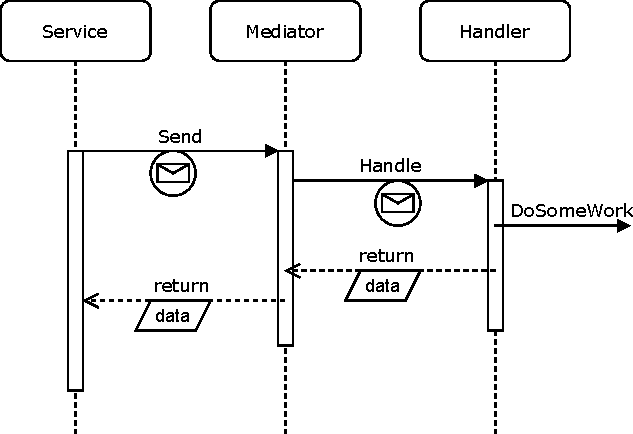
\includegraphics[width=.6\linewidth]{rys02/mediatR-Command-3.pdf}
	\caption{Przykład wysłania żądania}
	\label{fig:mediatR-Request}
\end{figure}

Zdarzenia różnią się od żądań tym, że mogą być przechwytywane przez wiele handlerów. Z tego też powodu nie można zwrócić rezultatu zdarzenia. W pewnym sensie można w wielu scenariuszach odpowiedzieć na zdarzenie publikacją innego zdarzenia (ang.~\emph{publish event}). Jest to nowoczesna technika, która umożliwia asynchroniczne wywoływanie innych funkcji systemu, w szczególności w architekturze \texttt{mikroserwisów} (ang.~\emph{micorservices architecture}). Przykład publikacji zdarzeń można zaobserwować na rysunku~\ref{fig:mediatR-Event}.

\begin{figure}[h]
	\centering
	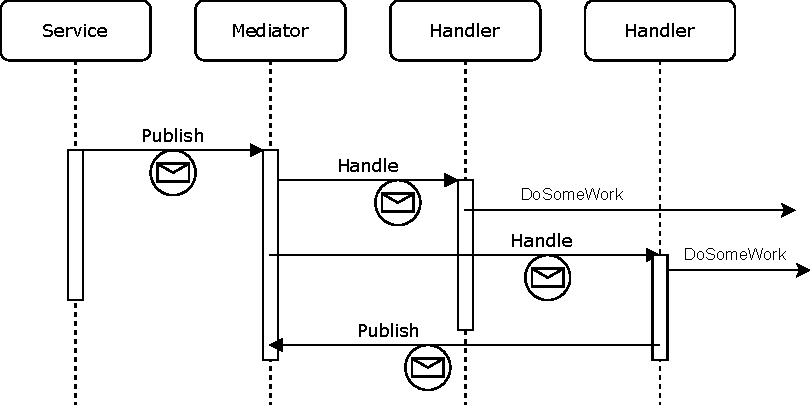
\includegraphics[width=.8\linewidth]{rys02/mediatR-notification-3.pdf}
	\caption{Przykład publikacji notyfikacji}
	\label{fig:mediatR-Event}
\end{figure}

\subsection{Podział odpowiedzialności czyli CQRS}
\label{subsec:cqrs}

Kolejnym wzorcem projektowym wartym uwagi w perspektywie tworzenia nowej aplikacji jest \texttt{CQRS} (ang.~\emph{Command Query Responsibility Segregation}). Pozwala on na użycie innego modelu do zapytań (ang.~\emph{queries}), czytających dane oraz do komend (ang.~\emph{command}), które modyfikują stan systemu. 

Na rysunku \ref{fig:cqrs-architecture} widać zarys architektury w przypadku bezstanowego API. Kierowane do API żądania HTTP GET przekazywane są do \emph{query} modelu, który czyta odpowiednie informację z bazy danych. Żądania POST przechwytuje \emph{command} model, posiadający skomplikowaną logikę biznesową, a następnie, jeśli reguły biznesowe na to pozwalają, aktualizuje dane w magazynie danych. Wartym uwagi jest fakt, że oba modele mogą korzystać z innych połączeń do bazy danych, a więc model dla zapytań może nawet nie mieć uprawnień do zapisu w bazie danych.

\begin{figure}[h]
	\centering
	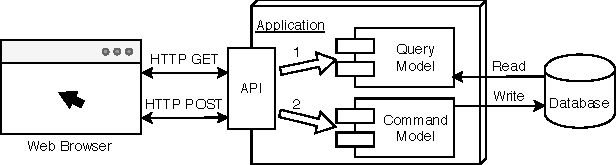
\includegraphics[width=.9\linewidth]{rys02/cqrs01.pdf}
	\caption{Architektura CQRS}
	\label{fig:cqrs-architecture}
\end{figure}

Gdy czytamy dane, często traktujemy aplikację serwerową jako opakowanie bazy danych -- swoisty kontener informacji~\cite{cqrs-fowler}. Najczęstszym, a także najważniejszym wymaganiem wobec zapytań jest ich wydajność. Natomiast podczas modyfikowania stanu systemu szybkość nie jest już krytycznym wymaganiem. Ważniejsze od niej są walidacja danych wejściowych, zgodność z regułami biznesowymi, obsługa wyjątków domenowych, a także atomowość operacji, tak aby pozostawić system w poprawnym stanie.

Segregacja komend i żądań pozwala dostosować kod źródłowy do specyficznych wymagań, jakie im się stawia. Rozdziela ona także odpowiedzialność klas na wyższym poziomie systemu -- warstwie aplikacji. Dzięki temu powstają klasy wyspecjalizowane klasy warstwy aplikacji, które wykonują zapytanie albo komendę. Mówi o tym także zasada pojedynczej odpowiedzialności\ref{chap:know-how}.

Ponadto CQRS idealnie komponuje się z systemem opartym o architekturę zdarzeń, którą oferuje, np. biblioteka MediatR, opisana w punkcie~\ref{subsec:mediator}. CQRS dobrze działa także w architekturach opartych o \emph{event sourcing} czy \texttt{DDD} (ang.~\emph{Domain Driven Design}), a których autor szerzej nie opisze w tej pracy.
\chapter{Założenia projektowe}
\label{chap:zalozenia-projektowe}
\section{Wymagania funkcjonalne}
\label{sec:wymagania-funkcjonalne}

W tej sekcji opisane zostaną wymagania funkcjonalne jakie powinien spełniać stworzony system. Zaprezentowane zostaną przypadki użycia dla czterech podsystemów: system zarządzania kontem pieniężnym, system zarządzania środkami finansowymi, system zarządzania rodziną i system zarządzania kategoriami. Przypadki użycia zostaną opisane w schemacie: nazwa przypadku użycia, aktor wykonujący akcję, warunki początkowe, warunki końcowe, cel oraz przebieg. Ponadto przypadki użycia zostaną zaprezentowane w formie diagramów.

\subsection{Wymagania dotyczące konta pieniężnego}
\label{subsec:wymagania-konto}
Poniżej opisano przypadki użycia dotyczące zarządzania kontem pieniężnym użytkownika. Zaprezentowano je także na diagramie (rys.~\ref{fig:use-case-account}).

\begin{enumerate}[labelwidth=1em,label=\arabic*.]
\item \textbf{Nazwa:} Dodaj konto \newline
    \textbf{Aktor:} Zalogowany użytkownik \newline
    \textbf{Warunki początkowe:} Użytkownik musi się wcześniej zarejestrować i być zalogowany w momencie tworzenia konta. \newline
    \textbf{Warunki końcowe:} Stan konta musi być zgodny z polityką dla jego typu. \newline
    \textbf{Cel:} Stworzenie w systemie konta pieniężnego przypisanego do aktora wykonującego tę operację, aby umożliwić zapisywanie informacji o przepływie gotówki. \newline
    \textbf{Przebieg:} Użytkownik wypełnia formularz. Wpisuje wymagane pola: nazwa konta, saldo początkowe i limit debetu oraz opcjonalne pola: numer konta, waluta i opis. Wybiera także typ konta.
\item \textbf{Nazwa:} Usuń konto \newline
    \textbf{Aktor:} Właściciel konta \newline
    \textbf{Warunki początkowe:} Użytkownik musi posiadać konto pieniężne. \newline
    \textbf{Warunki końcowe:} Użytkownik musi potwierdzić usunięcie konta. \newline
    \textbf{Cel:} Usunięcie konta pieniężnego użytkownika wraz z jego historią. \newline
    \textbf{Przebieg:} Użytkownik wybiera jedno ze swoich kont, a następnie naciska guzik usuń. Użytkownik musi potwierdzić tę operację.
\item \textbf{Nazwa:} Edytuj dane konta \newline
    \textbf{Aktor:} Właściciel konta \newline
    \textbf{Warunki początkowe:} Użytkownik musi posiadać konto pieniężne. \newline
    \textbf{Warunki końcowe:} Stan konta nie może przekraczać nowego limitu debetu. \newline
    \textbf{Cel:} Aktualizacja danych konta, bez utraty jego historii. \newline
    \textbf{Przebieg:} Użytkownik edytuje pola obowiązkowe formularza: nazwa konta, limit debetu oraz opcjonalne pola: numer konta, waluta i opis. Nie może edytować jego typu.
\item \label{last-item1}\textbf{Nazwa:} Zmień typ konta\newline
    \textbf{Aktor:} Właściciel konta \newline
    \textbf{Warunki początkowe:} Użytkownik musi posiadać konto pieniężne. \newline
    \textbf{Warunki końcowe:} Typ konta musi pozwalać na potencjalnie istniejący na koncie debet. \newline
    \textbf{Cel:} Zmiana typu konta na inny. Umożliwiające posiadanie debetu, lub oprocentowane. \newline
    \textbf{Przebieg:} Użytkownik po wybraniu konta zmienia jego typ, a swój wybór zatwierdza naciśnięciem guzika ,,Akceptuj''. 
\end{enumerate}

\begin{figure}[t]
	\centering
	\fbox{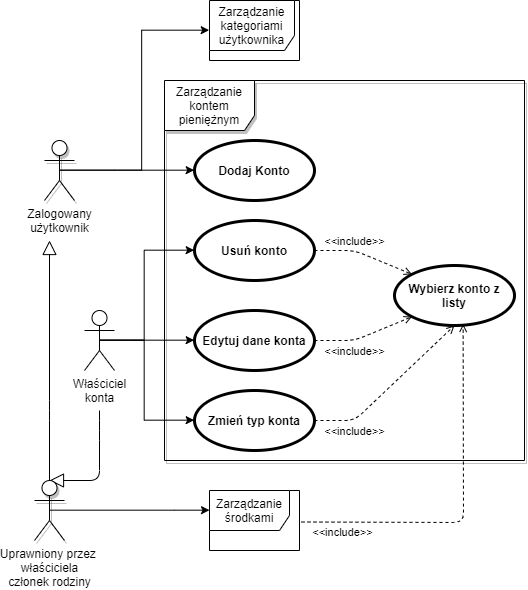
\includegraphics[width=.65\linewidth]{rys03/use-case-account.png}}
	\caption{Diagram przypadków użycia konta pieniężnego}
	\label{fig:use-case-account}
\end{figure}

\subsection{Wymagania dotyczące środków finansowych}
\label{subsec:wymagania-srodki-finansowe}
Na rysunku~\ref{fig:use-case-money} przedstawiono przypadki użycia związane z definiowaniem przepływu gotówki dla kont pieniężnych. Poniżej znajdują się także ich opisy.

\begin{enumerate}[labelwidth=1em,label=\arabic*.]
\item \textbf{Nazwa:} Dodaj wydatek/przychód \newline
    \textbf{Aktor:} Uprawniony przez właściciela członek rodziny \newline
    \textbf{Warunki początkowe:} Administrator rodziny zdefiniował co najmniej jedną kategorię dla operacji finansowych. \newline
    \textbf{Warunki końcowe:} Stan konta po operacji dodania wydatku musi być zgodny z polityką dla typu konta. \newline
    \textbf{Cel:} Zdefiniowanie operacji pieniężnej w ramach konta. \newline
    \textbf{Przebieg:} Użytkownik tworzy wydatek lub przychód wpisując obowiązkowe pola: kwota i data, a także te dodatkowe: notatka, odbiorca. Użytkownik musi także wybrać kategorię. 
\item \textbf{Nazwa:} Usuń wydatek/przychód \newline
    \textbf{Aktor:} Uprawniony przez właściciela członek rodziny \newline
    \textbf{Warunki początkowe:} Konto posiada co najmniej jeden wpis: wydatek lub przychód. \newline
    \textbf{Warunki końcowe:} Stan konta po operacji usunięcia przychodu musi być zgodny z polityką dla typu konta. \newline
    \textbf{Cel:} Usunięcie operacji pieniężnej w ramach konta. \newline
    \textbf{Przebieg:} Użytkownik wybiera wydatek lub przychód, a następnie naciska guzik usuń. 
\item \textbf{Nazwa:} Edytuj wydatek/przychód \newline
    \textbf{Aktor:} Uprawniony przez właściciela członek rodziny \newline
    \textbf{Warunki początkowe:} Konto posiada co najmniej jeden wpis: wydatek lub przychód. \newline
    \textbf{Warunki końcowe:} Stan konta po edycji wpisu musi być zgodny z polityką dla typu konta. \newline
    \textbf{Cel:} Edycja operacji pieniężnej w ramach konta. \newline
    \textbf{Przebieg:} Użytkownik wybiera wydatek lub przychód, a następnie naciska guzik ,,edytuj''. Edytuje pola obowiązkowe i dodatkowe. Jeśli chce zmienić kategorię musi ją wybrać z listy. \newline
    \textbf{Rozszerzenia: } 
    \begin{enumerate}[label=\alph*)]
        \item Użytkownik edytuje kategorię wpisu: Wybór kategorii.
    \end{enumerate}
\item \textbf{Nazwa:} Wykonaj przelew \newline
    \textbf{Aktor:} Uprawniony przez właściciela członek rodziny \newline
    \textbf{Warunki początkowe:} Administrator rodziny zdefiniował co najmniej jedną kategorię dla operacji finansowych. \newline
    \textbf{Warunki końcowe:} Stan konta po przelewie musi być zgodny z polityką dla typu konta. \newline
    \textbf{Cel:} Wykonanie przelewu między kontami lub zewnętrznego. \newline
    \textbf{Przebieg:} Użytkownik definiuje przelew wpisując obowiązkowe pola: kwota i data, a także dodatkowe: notatka, odbiorca. Użytkownik musi także wybrać kategorię. \newline
    \textbf{Rozszerzenia: }
    \begin{enumerate}[label=\alph*)]
        \item Użytkownik definiuje przelew między kontami rodziny: Przelew własny.
    \end{enumerate}
\end{enumerate}

\begin{figure}[t]
	\centering
	\fbox{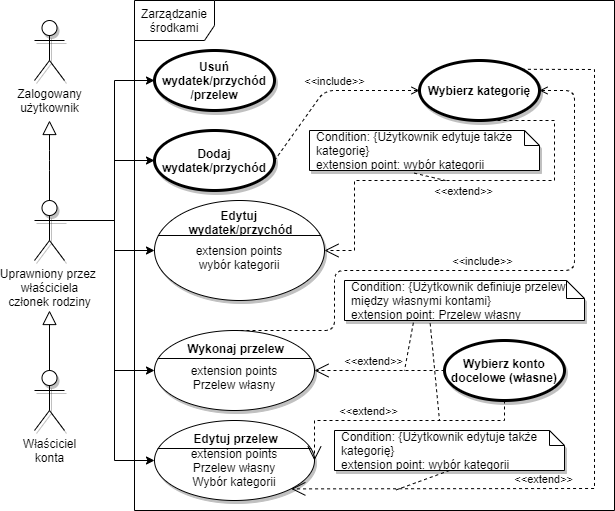
\includegraphics[width=.7\linewidth]{rys03/use-case-money.png}}
	\caption{Subdiagram przypadków użycia dla operacji finansowych}
	\label{fig:use-case-money}
\end{figure}

\subsection{Wymagania dotyczące rodziny}
\label{subsec:wymagania-rodzina}
Wymagania funkcjonalne dotyczące obsługi w aplikacji grupy rodziny, dalej zwanej rodziną, przedstawione zostały na~ rysunku~\ref{fig:use-case-family}. Poniżej znajdują się także ich szczegółowe opisy.

\begin{enumerate}[labelwidth=1em,label=\arabic*.]
\item \textbf{Nazwa:} Stwórz rodzinę \newline
    \textbf{Aktor:} Zalogowany użytkownik \newline
    \textbf{Warunki początkowe:} Użytkownik zarejestrował się w aplikacji. \newline
    \textbf{Warunki końcowe:} Użytkownik staje się administratorem nowoutworzonej rodziny. \newline
    \textbf{Cel:} Stworzenie rodziny, w ramach której można współdzielić konta pieniężne i ich historie. \newline
    \textbf{Przebieg:} Rodzina zostaje stworzona w momencie rejestracji. 
\item \textbf{Nazwa:} Akceptuj zaproszenie \newline
    \textbf{Aktor:} Zalogowany użytkownik \newline
    \textbf{Warunki początkowe:} Administrator innej rodziny dodał do niej użytkownika. \newline
    \textbf{Warunki końcowe:} Użytkownik zaakceptował zaproszenie.  \newline
    \textbf{Cel:} Dołączenie do nowej rodziny. \newline
    \textbf{Przebieg:} Użytkownik wyświetla zaproszenia do rodziny. Następnie akceptuje zaproszenie do jednej, bądź wielu z nich.
\item \textbf{Nazwa:} Dodaj członka \newline
    \textbf{Aktor:} Administrator rodziny \newline
    \textbf{Warunki początkowe:} Użytkownik stworzył rodzinę. \newline
    \textbf{Warunki końcowe:} Użytkownik akceptuje zaproszenie do rodziny.  \newline
    \textbf{Cel:} Dodanie nowego członka do rodziny, aby współdzielić historię finansową. \newline
    \textbf{Przebieg:} Administrator wpisuję login użytkownika, którego chce dodać i zatwierdza wybór guzikiem. 
\item \textbf{Nazwa:} Usuń członka \newline
    \textbf{Aktor:} Administrator rodziny \newline
    \textbf{Warunki początkowe:} Użytkownik dodał do rodziny co~najmniej jednego innego członka. \newline
    \textbf{Warunki końcowe:} --  \newline
    \textbf{Cel:} Usunięcie członka z rodziny. \newline
    \textbf{Przebieg:} Administrator naciska guzik usuń członka, a następnie potwierdza swoją akcję.
\item \textbf{Nazwa:} Edytuj uprawnienia dostępu do konta \newline
    \textbf{Aktor:} Członek rodziny będący właścicielem konta \newline
    \textbf{Warunki początkowe:} Użytkownik jest właścicielem konta. W rodzinie, do której przypisane jest konto jest więcej niż jeden członek. \newline
    \textbf{Warunki końcowe:} Właściciel konta potwierdza nadanie uprawnień naciskając guzik. \newline
    \textbf{Cel:} Nadanie uprawnień członkowi rodziny, aby mógł publikować wpisy w ramach konta i/lub przeglądać jego historię.  \newline
    \textbf{Przebieg:} Właściciel konta wybiera z listy jedno ze swoich kont w ramach rodziny. Następnie z listy wybiera członka rodziny, któremu chce nadać uprawnienia. Nadaje członkowi uprawnienia spośród: prawo do wglądu, prawo do dodawania wpisów.
    Swój wybór zatwierdza guzikiem ,,zatwierdź''.
\end{enumerate}

\begin{figure}[t]
	\centering
	\fbox{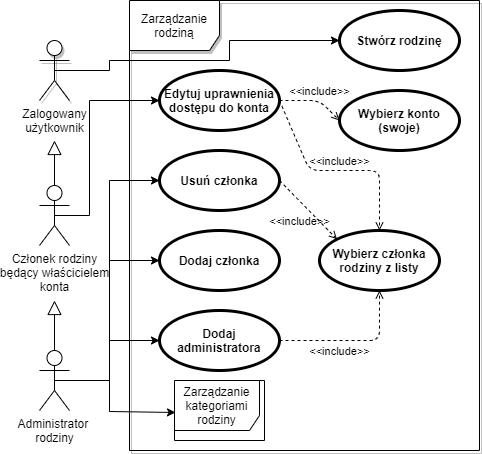
\includegraphics[width=.65\linewidth]{rys03/use-case-family.png}}
	\caption{Diagram przypadków użycia dla rodziny}
	\label{fig:use-case-family}
\end{figure}

\subsection{Wymagania dotyczące kategorii}
\label{subsec:wymagania-kategorie}

\begin{enumerate}[labelwidth=1em,label=\arabic*.]
\item \textbf{Nazwa:} Dodaj kategorię \newline
    \textbf{Aktor:} Zalogowany użytkownik \newline
    \textbf{Warunki początkowe:} Użytkownik zarejestrował się w aplikacji. \newline
    \textbf{Warunki końcowe:} Nazwa kategorii w swoim poddrzewie jest unikatowa. \newline
    \textbf{Cel:} Stworzenie kategorii, aby łatwiej segregować wydatki i przychody. \newline
    \textbf{Przebieg:} Użytkownik naciska guzik dodaj kategorię na drzewie kategorii. Następnie wpisuje jej nazwę i wybiera kolor wyświetlania wpisów przypisanych do niej.
\item \textbf{Nazwa:} Edytuj kategorię \newline
    \textbf{Aktor:} Zalogowany użytkownik \newline
    \textbf{Warunki początkowe:} Użytkownik dodał co najmniej jedną kategorię. \newline
    \textbf{Warunki końcowe:} Nazwa kategorii w swoim poddrzewie jest unikatowa. \newline
    \textbf{Cel:} Edycja istniejącej kategorii bez utraty historii wpisów tej kategorii. \newline
    \textbf{Przebieg:} Użytkownik edytuje nazwę i kolor kategorii. Może także przeciągnąć ją do innej kategorii nadrzędnej lub zrobić z niej kategorię najwyższego rzędu.
\item \textbf{Nazwa:} Ukryj kategorię \newline
    \textbf{Aktor:} Zalogowany użytkownik \newline
    \textbf{Warunki początkowe:} Użytkownik dodał co najmniej jedną kategorię. \newline
    \textbf{Warunki końcowe:} -- \newline
    \textbf{Cel:} Ukrycie istniejącej kategorii bez utraty historii wpisów tej kategorii. \newline
    \textbf{Przebieg:} Użytkownik w menu kategorii klika ukryj.
\item \textbf{Nazwa:} Usuń kategorię \newline
    \textbf{Aktor:} Zalogowany użytkownik \newline
    \textbf{Warunki początkowe:} Użytkownik dodał co najmniej jedną kategorię. Kategoria nie posiada żadnych wpisów. \newline
    \textbf{Warunki końcowe:} Nie istnieje wpis, który nie ma przypisanej kategorii. \newline
    \textbf{Cel:} Usunięcie kategorii, do której nie jest przypisany żaden wpis. \newline
    \textbf{Przebieg:} Użytkownik w menu kategorii klika usuń i zatwierdza wybór.
\end{enumerate}

\begin{figure}[t]
	\centering
	\fbox{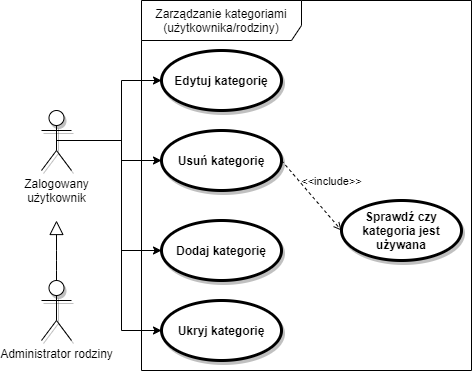
\includegraphics[width=.65\linewidth]{rys03/use-case-category.png}}
	\caption{Diagram przypadków użycia dla kategorii}
	\label{fig:use-case-category}
\end{figure}

\section{Wymagania niefunkcjonalne}
\label{sec:wymagania-niefunkcjonalne}

\begin{enumerate}[labelwidth=1em,label=\arabic*.]

\item System składać ma się z~dwóch głównych części:
\begin{enumerate}[label=\alph*)]
\item aplikacji serwerowej -- API. Jej zadaniem będzie dostarczanie interfejsu programistycznego do pobierania danych i~modyfikowania stanu systemu.
\item aplikacja webowej, dostarczająca graficzny interfejs użytkownika -- \texttt{GUI}. Aplikacja ta będzie konsumować API.
\end{enumerate}

\item Zarówno aplikacja webowa, jak i API będą stworzone przy pomocy frameworka ASP.NET Core w wersji co najmniej 2.2: 
\begin{enumerate}[label=\alph*)]
\item Do napisania aplikacji webowej użyte zostaną \texttt{Razor Pages} oraz komponenty widoku (ang.~\emph{view components}). 
\item Warstwa persystencji danych w aplikacji API stworzona zostanie z pomocą Entity Framework Core 2.2. Wykorzystane zostanie podejście \emph{code first} i mechanizm migracji.
\end{enumerate}

\item Pobieranie danych z API ma odbywać się za pomocą protokołu OData.

\item API używać będzie bazy danych na serwerze Microsoft SQL Server 2017 (lub nowszym).

\item Aplikacja webowa powinna poprawnie działać co najmniej w przeglądarkach: Mozilla Firefox, Google Chrome, Opera, Microsoft Edge oraz Safari, a~także przeglądarkach mobilnych: Opera Mobile, Google Chrome, Mozilla Firefox i Safari.

\item Aplikacja będzie wymuszać działanie z wykorzystaniem protokołu \texttt{HTTPS} (ang.~\emph{Hypertext Transfer Protocol Secure}).

\item Autoryzacja i uwierzytelnienie ma być przeprowadzona z wykorzystaniem protokołu OpenId Connect i frameworka autoryzacji OAuth 2.0. Użyty powinien zostać \emph{Hybrid Flow} lub \emph{Authorization Code Flow}.

\item Dostawcą tożsamości w systemie powinna być osobna aplikacja, posiadająca własną bazę danych lub zewnętrzy system autoryzacji, np.~\texttt{Auth0}.

\item API ma posiadać dokumentację stworzoną przy pomocy narzędzia \texttt{Swagger}.

\item Kod źródłowy ma być napisany z wykorzystaniem dobrych praktyk programowania~i~wzorców projektowych ułatwiających jego utrzymanie i rozwijanie.

\item System działać będzie na platformie chmurowej \texttt{Microsfot Azure}.

\item Poszczególne składowe systemu w chmurze powinny być automatycznie skalowalne.

\item Aplikacja webowa powinna być bezpieczna i odporna na ataki. Zostanie wykorzystany mechanizm obrony przed \texttt{CSRF} (ang.~Cross-Site Request Forgery) -- \texttt{anti-forgery token}.

\end{enumerate}

\section{Metodyka}
\label{sec:metodyka}*
\chapter{Implementacja}
\label{chap:implementacja}

\section{Struktura projektu}
\label{sec:struktura-projektu}
W tym podrozdziale przedstawiono logiczną i fizyczną strukturę projektu. Uwzględniono przy tym podział na projekty aplikacji klienckiej oraz API, gdyż stanowią one tak na prawdę niezależne rozwiązania (ang.~\emph{solution}) w środowisku programistycznym Visual Studio 2019.

\subsection{Struktura fizyczna projektu}
\label{sec:struktura-fizyczna-projektu}
Obie aplikacje (aplikacja kliencka i API) znajdują się w tym samym repozytorium Git. Pliki ich rozwiązań znajdują się w folderze głównym repozytorium. W folderze tym znajduję się także plik \texttt{.gitignore}. Projekty należące do rozwiązań znajdują się w folderze \texttt{src}. W katalogu \texttt{Zoltaniecki.IDP} znajduję się potrzebny do testów dostawca tożsamości, będący tylko wydmuszką prawdziwego serwisu. Strukturę głównego folderu można zobaczyć na rysunku~\ref{fig:fiz-1}.
\begin{figure}[ht]
	\centering
	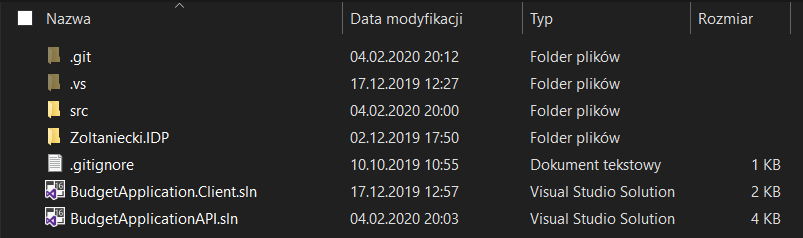
\includegraphics[scale=.77]{rys04/struktura-fizyczna-1.PNG}
	\caption{Struktura fizyczna repozytorium}
	\label{fig:fiz-1}
\end{figure}

W folderze \texttt{src} znajdują się dwa następne foldery: \texttt{API} oraz \texttt{Client}. Znajdują się w nich kolejno projekty dla rozwiązania: \texttt{BudgetApplicationAPI.sln} i~dla rozwiązania \texttt{BudgetApplicationClient.sln} (rys.~\ref{fig:fiz-2}). 
%todo czy usunać?
\begin{figure}[ht]
	\centering
	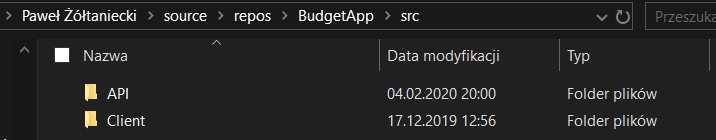
\includegraphics[scale=.77]{rys04/struktura-fizyczna-2.PNG}
	\caption{Zawartość folderu src}
	\label{fig:fiz-2}
\end{figure}

Warto zwrócić uwagę, że zarówno w API jak i w aplikacji klienckiej klasy pogrupowane są według funckjonoalności, a nie typów np.: \texttt{Services}, \texttt{Controllers}, \texttt{Views}, \texttt{Models}. Daje to dużą elastyczność i wygodę przy pracy programisty, gdyż nie musi szukać klas związanych z~jedną funkcjonalnościach w wielu w poddrzewach katalogów.

\subsubsection{Fizyczna struktura API}
Aplikacja API składa się z czterech projektów (rys.~\ref{fig:fiz-api-2}): \texttt{BudgetApplication.API}, \texttt{BudgetApplication.Domain}, \texttt{BudgetApplication.Infrastructure} oraz \texttt{BudgetApplication.QueryInfrastructure} umieszczonych w osobnych folderach. % (rys.~\ref{fig:fiz-api-1})
%%%todo czy usunać?
%%\begin{figure}[ht]
	%%\centering
	%%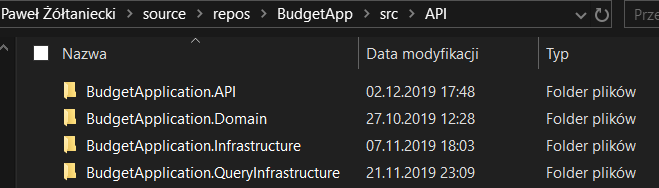
\includegraphics[scale=.77]{rys04/struktura-fizyczna-api-1.PNG}
	%%\caption{Zawartość folderu API}
	%%\label{fig:fiz-api-1}
%%\end{figure}
%Na rysunku~\ref{fig:fiz-api-2} przedstawiono strukturę rozwiązania dla API. Widać na nim cztery projekty zawierające różne foldery. 
\begin{figure}[ht]
	\centering
	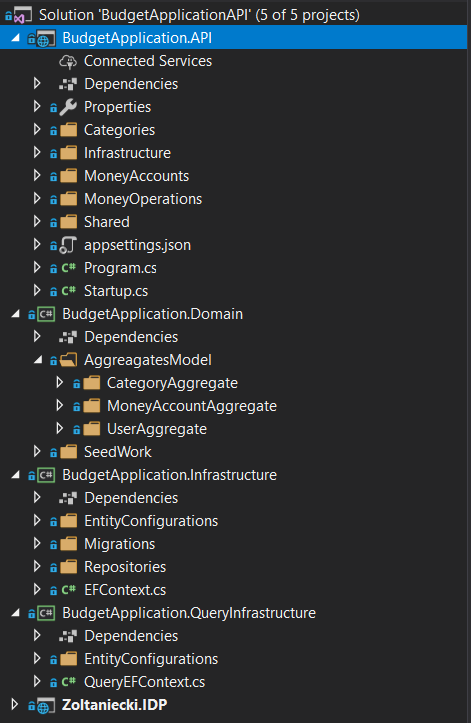
\includegraphics[scale=.77]{rys04/struktura-fizyczna-api-2.PNG}
	\caption{Struktura rozwiązania API}
	\label{fig:fiz-api-2}
\end{figure}

Foldery projektu \texttt{API} zawierają pogrupowane według funkcjonalności klasy kontrolerów API (ang.~\emph{controllers}), a także klasy związane z opisaną w sekcji~\ref{subsec:mediator} biblioteką \texttt{MediatR}: handlery (ang.~\emph{handlers}), komendy (ang.~\emph{commands}) i odpowiedzi(ang.~\emph{responses}). Katalog \texttt{Shared} zawiera współdzielone interfejsy. 

W projekcie \texttt{Domain} podkatalogi katalogu \texttt{AggregatesModel} zawierają pogrupowane według funkcjonalności encje, ich serwisy domenowe, klasy wyjątków domenowych, enumeratory, klasy typu \texttt{DTO} (ang.~\emph{Data transfer object}), a także inne klasy związane z przetwarzaniem logiki biznesowej. Folder \texttt{SeedWork} zawiera związane z taktycznym DDD interfejsy i klasy bazowe. \texttt{Program.cs} zawiera funkcję \texttt{Main}, czyli punkt wejścia do programu, a w klasie \texttt{Startup} konfigurowana jest aplikacja i jej serwisy.

Projekty \texttt{Infrastructure} i \texttt{QueryInfrastructure} zawierają warstwę dostępu do danych kolejno dla komend i zapytań, związanych z zastosowanym wzorcem \texttt{CQRS}, opisanym w punkcie~\ref{subsec:cqrs}. Foldery \texttt{EntityConfigurations} zawierają mapowania relacyjno-obiektowe charakterystyczne dla Entity Framework Core. Folder \texttt{Repositories} zawiera implementacje wzorca repozytorium dla klas encji biznesowych. Natomiast katalog \texttt{Migrations} zawiera pliki migracji modelu w bazie danych.


\subsubsection{Fizyczna struktura aplikacji klienckiej}

Aplikacja kliencka składa się z dwóch projektów (rys.~\ref{fig:fiz-client-2}): \texttt{BudgetApplication.Client} oraz \texttt{BudgetApplication.Client.Core} umieszczonych w osobnych folderach. 
%%\begin{figure}[ht]
	%%\centering
	%%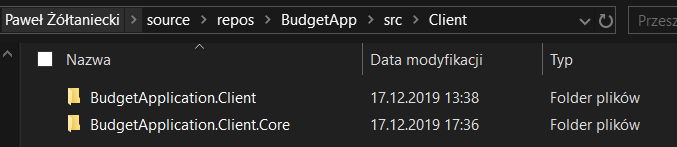
\includegraphics[scale=.77]{rys04/struktura-fizyczna-client-1.PNG}
	%%\caption{Zawartość folderu Client}
	%%\label{fig:fiz-client-1}
%%\end{figure}
%Na rysunku~\ref{fig:fiz-client-2} przedstawiono strukturę rozwiązania aplikacji klienckiej.
\begin{figure}[htb]
	\centering
	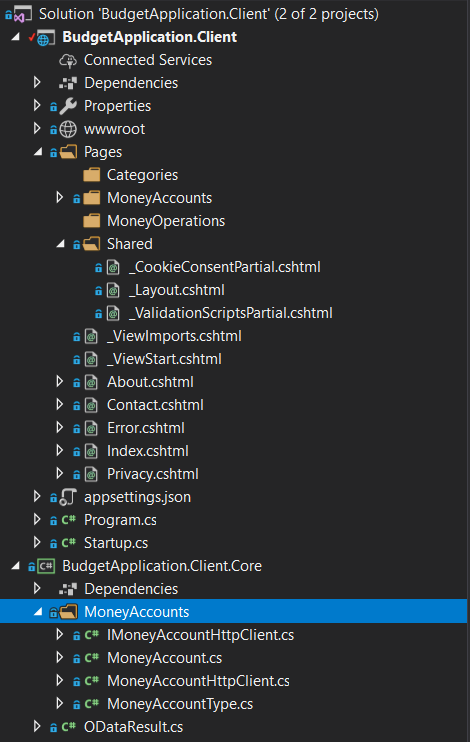
\includegraphics[scale=.77]{rys04/struktura-fizyczna-client-2.PNG}
	\caption{Struktura rozwiązania aplikacji klienckiej}
	\label{fig:fiz-client-2}
\end{figure}

Pierwszy z projektów zawiera jeden główny folder z widokami i ich modelami strony (ang.~\emph{page model}), pogrupowanymi w foldery według funkcjonalności. W głównym folderze znajdują się też widoki niezwiązane z modelami strony, a także folder \texttt{Shared} z widokami częściowymi używanymi przez pozostałe widoki. Pliki: \texttt{Program.cs} i \texttt{Startup.cs} pełnią podobną funkcję co w projekcie API.

Drugi z projektów, także zawiera tylko jeden główny katalog. Zawiera on odpowiednio skonfigurowane klasy klientów HTTP, komunikujące się z API, a także klasy modeli, które są zwracane przez zakończone sukcesem żądania HTTP.

Klasa \texttt{ODataResult} jest klasą odpowiedzi żądań HTTP GET. Zawiera ona właściwości takie jak: \emph{Count}, \emph{Metadata}, \emph{Context} i \emph{Value}, ściśle związana z implementacją protokołu OData -- punkt~\ref{subsec:odata}. Pole Value jest polem generycznym w zależności od zwracanego przez żądanie HTTP modelu. 


\subsection{Struktura logiczna projektu}
\label{sec:struktura-logiczna-projektu}
Poniżej zaprezentowano logiczną strukturę projektu. Pokazano też zależności między projektami zawartymi w rozwiązaniach dla aplikacji klienckiej oraz API.

\subsubsection{Logiczna struktura API}
Aplikacja API składa się z czterech projektów: \texttt{BudgetApplication.API}, \texttt{BudgetApplication.Domain}, \texttt{BudgetApplication.Infrastructure} oraz \texttt{BudgetApplication.QueryInfrastructure} z zależnościami jak na rysunku~\ref{fig:api-arch}. 
\begin{figure}[ht]
	\centering
	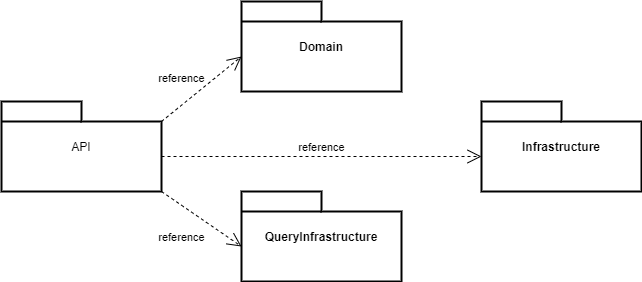
\includegraphics[scale=.55]{rys04/api-arch.png}
	\caption{Zależności między projektami w API}
	\label{fig:api-arch}
\end{figure}

Projekt \texttt{API} zawiera API kontrolery, a także handlery, odpowiedzi i żądania MediatR. Razem składają się one na warstwę aplikacji. Warstwa aplikacji operuje na obiektach domenowych, dlatego też projekt \texttt{API} zależny jest od projektu \texttt{Domain}.

Projekt \texttt{Domain} jest projektem ślepym i nie ma żadnych zależności. Znajduje się w nim kod niezależny od innych zewnętrznych frameworków. Definiuje on zachowania biznesowe obiektów domenowych, które są używane podczas wykonywania komend CQRS, wcześniej opisanych w punkcie~\ref{subsec:cqrs}. Model domenowy jest szczególnie istotny z punktu widzenia zachowania prawidłowego stanu systemu w trakcie i po wykonaniu operacji.

Warstwę persystencji dla encji domenowych stanowi projekt \texttt{Infrastructure}. Znajdują się w nim m.in. repozytoria, które implementują kontrakt zdefiniowany w projekcie \texttt{Domain}. Repozytoria korzystają z mapera relacyjno-obiektowego Entity Framework Core. Ten projekt tworzony jest dla zachowania niezależności domeny od zewnętrznych frameworków.

Projekt \texttt{QueryInfrastructure} to projekt dostarczający uproszczoną wersję modelu zapisanego w bazie danych, bez logiki domenowej. Obiekty tworzone w tej części aplikacji potrzebne są dla wykonania zapytań CQRS -- punkt~\ref{subsec:cqrs}. Projekt stworzono, podobnie jak poprzedni, również z wykorzystaniem Entity Framework Core. Oba projekty są niezależne i nic nie stoi na~przeszkodzie, aby zamiast EF Core wykorzystać technologię wbudowaną w Net Framework -- ADO.NET czy bibliotekę innego mapera relacyjno-obiektowego -- \texttt{Dapper}.

\subsubsection{Logiczna struktura aplikacji klienckiej}

Aplikacja kliencka składa się z dwóch projektów: \texttt{BudgetApplication.Client} oraz \texttt{BudgetApplication.Client.Core} z zależnościami jak na rysunku~\ref{fig:client-arch}.

\begin{figure}[ht]
	\centering
	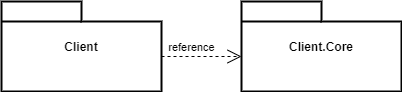
\includegraphics[scale=.55]{rys04/client-arch.png}
	\caption{Zależności między projektami w aplikacji klienckiej}
	\label{fig:client-arch}
\end{figure}

Projekt \texttt{Client} zawiera strony Razor Pages, które odpowiedzialne są za prezentowanie danych użytkownikowi i zapewnianie mu interfejsu do dokonywania zmian w systemie.

\texttt{Client.Core} zawiera klasy odpowiedzialne za komunikację z API i dostarczanie danych potrzebnych na stronach aplikacji.


\section{Szczegóły implementacji}
\label{sec:szczegoly-implementacji}
W tym podrozdziale opisano szczegóły implementacji API oraz aplikacji klienckiej. 

\subsection{Szczegóły implementacji API}
\label{subsec:szczegoly-implementacji-api}
Żądania HTTP wysłane do API przechodzą przez moduł routingu (ang.~\emph{Routing Middleware}) frameworka ASP.NET MVC. To on decyduje, do którego kontrolera i do jakiej jego akcji skierować żądanie. Jest to szczególnie istotne w bardziej skomplikowanych scenariuszach. Jednym z takich scenariuszy jest używanie implementacji protokołu OData równocześnie z routingiem atrybutowym (ang.~\emph{attribute routing}). Aby dodać routing OData do API, wystarczy w metodzie \texttt{Configure} klasy \texttt{Startup} dodać kod widoczny na listingu~\ref{list:odata-route-config}. Konfiguruje on prefix ścieżki do zasobów OData na \texttt{/api/odata}. Umożliwia on także na używanie selekcji, filtrowania, sortowania, zliczania, a także rozszerzania i stronicowania zasobu OData. 

Metoda \texttt{GetEdmModel} buduje model OData na podstawie klas encji przechowywanych w~bazie danych. Model mapowany jest do dalszej części ścieżki zasobów adresu URL za pomocą parametru przekazywanego do metody \texttt{EntitySet}. Wartość tego parametru musi być taka sama jak atrybut routingu w kontrolerze OData. Na podstawie modelu EDM generowane są metadane dla zasobów. 

{\belowcaptionskip=-10pt
\begin{lstlisting}[label=list:odata-route-config,
    caption=Konfiguracja rouingu OData w aplikacji MVC]
app.UseMvc(routeBuilder =>
{
    AddOdataRoutes(routeBuilder);
});
...
private static void AddOdataRoutes(Microsoft.AspNetCore.Routing.IRouteBuilder routeBuilder)
{
    routeBuilder.EnableDependencyInjection();
    routeBuilder.Select().Filter().OrderBy().Count().Expand().MaxTop(100).SkipToken();
    routeBuilder.MapODataServiceRoute("odata", "api/odata", OdataExtensionsMethods.GetEdmModel());
}
...
internal static IEdmModel GetEdmModel()
{
    var builder = new ODataConventionModelBuilder();

    builder.EntitySet<Category>("categories");
    builder.EntitySet<MoneyAccount>("money-accounts");
    builder.EntitySet<MoneyOperation>("money-operations");
    builder.EntitySet<Expense>("expenses");
    builder.EntitySet<Income>("incomes");

    return builder.GetEdmModel();
}
\end{lstlisting}
}

Kontroler OData i standardowy kontroler API różnią się od siebie pod kilkoma względami. Standardowy kontroler API dziedziczy po klasie \texttt{ControllerBase} i używa atrybutów routingu \texttt{Route} z przestrzeni nazw \texttt{Microsoft.AspNetCore.Mvc}. Natomiast kontroler OData dziedziczy po klasie \texttt{ODataController}. Dzięki zastosowaniu klasy \texttt{ODataController} kontroler OData m.in.~zwraca dane w~formacie zgodnym z protokołem OData, czyli opakowuje dane w~pole \texttt{values}, zapewnia link do metadanych zasobu, a także odpowiednie nagłówki charakterystyczne dla protokołu. Kontroler OData używa także innych atrybutów routingu: \texttt{ODataRoute} dla pojedynczej akcji oraz \texttt{ODataRoutePrefix} dla określenia prefixu routingu dla wszystkich akcji kontrolera. Znajdują się one w przestrzeni nazw \texttt{Microsoft.AspNet.OData.Routing}. Zastosowanie nieodpowiednich atrybutów routingu skutkuje błędem dopasowania wielu akcji do jednego adresu (ang.~\emph{AmbiguousActionException: Multiple actions matched}) lub zwróceniem statusu HTTP 404. Na listingu~\ref{list:api-ctrl-1} oraz~\ref{list:odata-ctrl-1} przedstawiono przykłady implementacji obu kontrolerów. Część kodu została pominięta dla klarowności.

Ponadto w kontrolerze OData używane są atrybuty \texttt{EnableQuery}. Zezwalają one na korzystanie w adresie URL z opcji filtrowania, sortowania itd., skonfigurowanych w metodzie \texttt{AddOdataRoutes} na listingu~\ref{list:odata-route-config}. Brak tych atrybutów dla konkretnej akcji skutkować będzie brakiem obsługi tych funkcjonalności. Ścieżka wyszukiwania (ang.~\emph{query string} będzie w tym wypadku ignorowana. Istnieje też atrybut \texttt{Queryable}, który można wykorzystać do ograniczenia funkcjonalności, które programista chce udostępnić w akcji. Robi się to za pomocą przekazania do atrybutu podzbioru skonfigurowanych opcji wyszukiwania OData. Tutaj przykład atrybutu ograniczającego opcje wyszukiwania do stronicowania: \texttt{[Queryable(AllowedQueryOptions=
    AllowedQueryOptions.Skip | AllowedQueryOptions.Top)]}

{\belowcaptionskip=-10pt
\begin{lstlisting}[label=list:api-ctrl-1,
    caption=Przykład implementacji standardowego kontrolera API]
[Route("api/money-accounts")]
[ApiController]
public class MoneyAccountsController : ControllerBase
{
    private readonly IMediator _mediator;
...
    //Patch api/money-accounts/1
    [HttpPatch]
    [Route("{moneyAccountId}")]
    public async Task<IActionResult> UpdateAccount(Guid moneyAccountId,
        UpdateMoneyAccountCommand updateMoneyAccountCommand)
    {
        updateMoneyAccountCommand.MoneyAccountId = moneyAccountId;
        bool result = await _mediator.Send(updateMoneyAccountCommand);
    
        if (!result)
        {
            return BadRequest();
        }
    
        return Ok();
    }
}
\end{lstlisting}
}

{\belowcaptionskip=-10pt
\begin{lstlisting}[label=list:odata-ctrl-1,
    caption=Przykład implementacji kontrolera OData]
[ODataRoutePrefix("money-accounts")]
public class ODataMoneyAccountController : ODataController
{
    private readonly QueryEFContext _moneyAccountRepository;
...
    [EnableQuery]
    [ODataRoute("{id}")]
    public ActionResult<MoneyAccount> GetAsync(Guid id)
    {
        return Ok(_moneyAccountRepository.MoneyAccounts
            .Where(acc => acc.Id == id));
    }
}
\end{lstlisting}
}

W systemie aplikacji domowego budżetu kontrolery OData są używane tylko do żądań HTTP GET, a kontrolery API do wszystkich innych żądań, które zmieniają stan systemu.
Kontroler OData bezpośrednio korzysta z kontekstu do bazy danych, który zwraca kolekcję implementują generyczny interfejs \texttt{IQueryable}. Dzięki temu OData jest w stanie przenieść logikę zapytania do bazy danych.

Standardowy kontroler API korzysta z mediatora, aby wysłać komendę do kolejnej warstwy aplikacji, w której zachodzą procesy biznesowe. Przykład serwisu aplikacji, który przetwarza komendę pokazano na listingu~\ref{list:handler-impl}. Operuje on na encjach i serwisach domenowych. W tym wypadku wykorzystano repozytorium do pobrania konta bankowego z bazy danych. Następnie do konta bankowego dodawany jest nowy wydatek, a całość zapisywana jest z zastosowaniem wzorca \texttt{Unit of Work}, który gwarantuje, że zmiany, które zaszły w systemie będą zapisane w~jednej transakcji bazodanowej. 

{\belowcaptionskip=-10pt
\begin{lstlisting}[label=list:handler-impl,
    caption=Przykład implementacji handlera aplikacji]
public async Task<CreateExpenseResponse> Handle(CreateExpenseCommand command, CancellationToken cancellationToken)
{
    var accountId = command.AccountId;
    var expenseDTO = _mapper.Map<AddExpenseDTO>(command);
    MoneyAccount moneyAccount = await _moneyAccountRepository.GetAsync(accountId);

    IReadOnlyExpense operation = moneyAccount.AddOperation(expenseDTO);

    _moneyAccountRepository.Update(moneyAccount);
    bool success = await _moneyAccountRepository.UnitOfWork.SaveEntitiesAsync();

    return success ? _mapper.Map<CreateExpenseResponse>(operation) : null;
}
\end{lstlisting}
}

\subsection{Szczegóły implementacji aplikacji klienckiej}
\label{subsec:szczegoly-implementacji-client}

Żądania użytkownika wysyłane do aplikacji klienckiej mapowane są do konkretnych stron Razor Pages. Strona Razor Page składa się z widoku napisanego przy pomocą języka html i opcjonalnie modelu strony (ang.~\emph{page model}). Na stronie często też znajdują się dodatkowe komendy składni Razor, których zadaniem jest budowanie widoku w zależności od modelu przekazanego do strony, a także generowanie widoków częściowych (ang.~\emph{partial views}). Widoki częściowe ułatwiają wydzielanie wspólnych części widoku strony do oddzielnych plików. Można łatwo wykorzystać je w różnych stronach Razor, a także użyć w pętli dla kolekcji obiektów zawartych w modelu widoku. Widoki częściowe nie mogą mieć swoich modeli strony, a jedynie polegają na danych przekazanych do nich z zewnątrz.

Aby widok był stroną Razor Page musi na nim znaleźć się dyrektywa \texttt{@page}. Służy ona także do routingu w aplikacji. Domyślnie routing oparty jest o strukturę folderów i nazwę strony. Oczywiście w takiej formie jest niewystarczający. Na listingu~\ref{list:razor-page-1} pokazano przykład wykorzystania dyrektywy \texttt{@page} do stworzenia strony konta bankowego o konkretnym identyfikatorze typu \texttt{guid} -- linia 1.

{\belowcaptionskip=-10pt
\begin{lstlisting}[label=list:razor-page-1,
    caption=Przykład strony Razor Page: \texttt{Edit.cshtml}]
@page "{accountId:guid?}"
@model BudgetApplication.Client.Pages.MoneyAccounts.EditModel
...
<h2>Edycja konta: @Model.MoneyAccount.Name</h2>
@if (Model.Message != null)
{
    <div class="alert alert-info">@Model.Message</div>
}
<form method="post">
  <input type="hidden" asp-for="MoneyAccount.Id" />

  <div class="form-group">
    <label asp-for="MoneyAccount.Name"></label>
    <input asp-for="MoneyAccount.Name" class="form-control" />
    <span asp-validation-for="MoneyAccount.Name" class="text-danger"></span>
  </div>
  ...
  <div class="form-group">
    <label asp-for="MoneyAccount.Type"></label>
    <select asp-for="MoneyAccount.Type" asp-items="Model.MoneyAccountTypes" class="form-control"></select>
    <span asp-validation-for="MoneyAccount.Type" class="text-danger"></span>
  </div>
  ...
</form>
@section Scripts {
    <partial name="_ValidationScriptsPartial" />
}
\end{lstlisting}
}

Na listingu~\ref{list:razor-page-1} pokazano także, w jaki sposób za pomocą składni Razor napełnić widok danymi z modelu strony. Przykładem takiej dyrektywy jest ta w linijce 4. Dyrektywy używające modelu strony mogą posłużyć także do warunkowego generowania części widoku -- linie 5-7.

Strona z listingu~\ref{list:razor-page-1} zawiera dyrektywę Razor \texttt{@model}. Określa ona typ modelu strony przypisanego do strony. Jego nazwa składa się z nazwy strony i doklejonego do niej przyrostka \texttt{Model}. Model strony jest ściśle powiązany ze stroną. Jest tzw. klasą ,,code-behind''. Pomiędzy widokiem strony Razor i modelem strony jest wiązanie, które sprawia, że zmiany na widoku odzwierciedlane są w modelu, a zmiany w modelu odzwierciedlane są na stronie. Ten proces ma miejsca poprzez synchroniczne żądania HTTP, w trakcie działań użytkownika, takich jak: wejście na stronę, odświeżenie strony, naciśnięcie guzika. Jest to realizacja popularnego wzorca architektonicznego \texttt{MVVM} (ang.~\emph{Model–view–viewmodel}).

Model strony to klasa dziedzicząca po klasie \texttt{PageModel}. Implementuje on dwie metody: \texttt{OnGetAsync} oraz \texttt{OnGetAsync}. W pierwszej z nich implementowana jest logika pobierania danych i napełniania nimi widoku strony. Druga z nich służy do obsługi żądań HTTP POST użytkownika, a w szczególności do wysyłania formularzy. 

Na listingu~\ref{list:razor-page-model-1} przedstawiono przykład modelu strony. Zawiera on właściwość typu \texttt{MoneyAccount}. Pola jej klasy są bezpośrednio mapowane na wartości za pomocą dyrektyw Razor w pliku strony -- listing~\ref{list:razor-page-1}. W metodzie \texttt{OnGetAsync} przypisywany jest obiekt konta bankowego do tej właściwości. Warto zwrócić uwagę, że zarówno parametr metody \texttt{OnGetAsync}, jak i parametr dyrektywy routingu \texttt{@page} (listing~\ref{list:razor-page-1} linia 1) mają typ mogący być wartością \texttt{null}. Dzięki temu strona obsługuje dwie ścieżki routingu: \texttt{/Edit/{id}} do strony edycji istniejącej konta bankowego o podanym id oraz \texttt{/Edit} do strony tworzenia nowego konta bankowego. Podobna sytuacja ma miejsce w metodzie \texttt{OnPostASync}.

Atrybut \texttt{[BindProperty]} dla właściwości \texttt{MoneyAccount} sprawia, że konto bankowe tworzone jest na podstawie danych z żądania i od razu przypisywane do właściwości, dlatego metoda \texttt{OnPostAsync} nie musi mieć parametru typu \texttt{MoneyAccount}. Domyślnie ten atrybut działa tylko dla żądania POST, jednak łatwo go skonfigurować dla żądań GET. W tym przykładzie jest to niepotrzebne.

Za pomocą metody \texttt{GetEnumSelectList} tzw.\ ,,Tag Helper'', łatwo zmapowowano wartości enumeratora \texttt{MoneyAccountType} na kolekcję, wykorzystywaną w rozwijanym menu w formularzu na listingu~\ref{list:razor-page-1} - linia 18-21.

{\belowcaptionskip=-10pt
\begin{lstlisting}[label=list:razor-page-model-1,
    caption=Przykład modelu strony Razor Page: \texttt{EditPage.cs}]
public class EditModel : PageModel
{
...
  [BindProperty]
  public MoneyAccount MoneyAccount { get; set; }
  public IEnumerable<SelectListItem> MoneyAccountTypes { get; set; }
  public async Task<IActionResult> OnGetAsync(Guid? accountId)
  {
    MoneyAccountTypes = _htmlHelper.GetEnumSelectList<MoneyAccountType>();
    if (accountId.HasValue)
      MoneyAccount = await _accountHttpClient.GetMoneyAccountByIdAsync(accountId.Value);
    else
      MoneyAccount = new MoneyAccount();
    
    return MoneyAccount == null 
      ? RedirectToPage("./NotFound")
      : Page() as IActionResult;
  }

  public async Task<IActionResult> OnPostAsync()
  {
    if (!ModelState.IsValid)
    {
      MoneyAccountTypes = _htmlHelper.GetEnumSelectList<MoneyAccountType>();
      return Page();
    }
    try
    {
      MoneyAccount = MoneyAccount.Id == Guid.Empty 
        ? await _accountHttpClient.AddMoneyAccountsAsync(MoneyAccount)
        : await _accountHttpClient.EditMoneyAccountsAsync(MoneyAccount);

      return RedirectToPage("./Edit", new { accountId = MoneyAccount.Id });
    }
    ...
  }
}
\end{lstlisting}
}

Na końcu listingu~\ref{list:razor-page-1} znajduje się dyrektywa generująca widok częściowy w sekcji \texttt{Scripts} głównego układu strony -- plik \texttt{\_Layout.cshtml}. Odpowiada ona za generowanie na stronie \texttt{Edit.cshtml} skryptów biblioteki \texttt{jQuery unobtrusive validation}, która współpracuje z~frameworkiem ASP.NET Core i zapewnia walidację po stronie klienta na podstawie adnotacji modelu klasy języka C\#. 

Przykład walidowanej klasy znajduje się na listingu~\ref{list:razor-validation-1}. Przed tagiem \texttt{body} HTML w~pliku \texttt{\_Layout.cshtml} znajduje się dyrektywa \texttt{@RenderSection("{}Scripts", required: false)}. Umożliwia dołączenie opcjonalnej sekcji skryptów przez widoki, korzystające z tego układu strony.


{\belowcaptionskip=-10pt
\begin{lstlisting}[label=list:razor-validation-1,
    caption=Przykład klasy z adnotacjami]
using System.ComponentModel.DataAnnotations;
public class MoneyAccount
{
    public Guid Id { get; set; }
    [Required]
    public Guid UserId { get; set; }
    [Required, MinLength(8)]
    public string Name { get; set; }
    [Required]
    public MoneyAccountType Type { get; set; }
    [MaxLength(255)]
    public string Description { get; set; }
...
    [MinLength(26)]
    [MaxLength(26)]
    public string BankAccountNumber { get; set; }
}
\end{lstlisting}
}

\subsection{Strony aplikacji klienckiej}
\label{subsec:widok-client}

W tym punkcie przedstawione są niektóre widoki z aplikacji klienckiej. Na pierwszym z nich -- rysunek~\ref{fig:ss-6}, przedstawiono widok listy kont pieniężnych użytkownika. Oferuję on możliwość dodanie nowego konta, jak i również wykonania akcji edycji, usunięcia i przejrzenia informacji o wybranym koncie.

\begin{figure}[ht]
	\centering
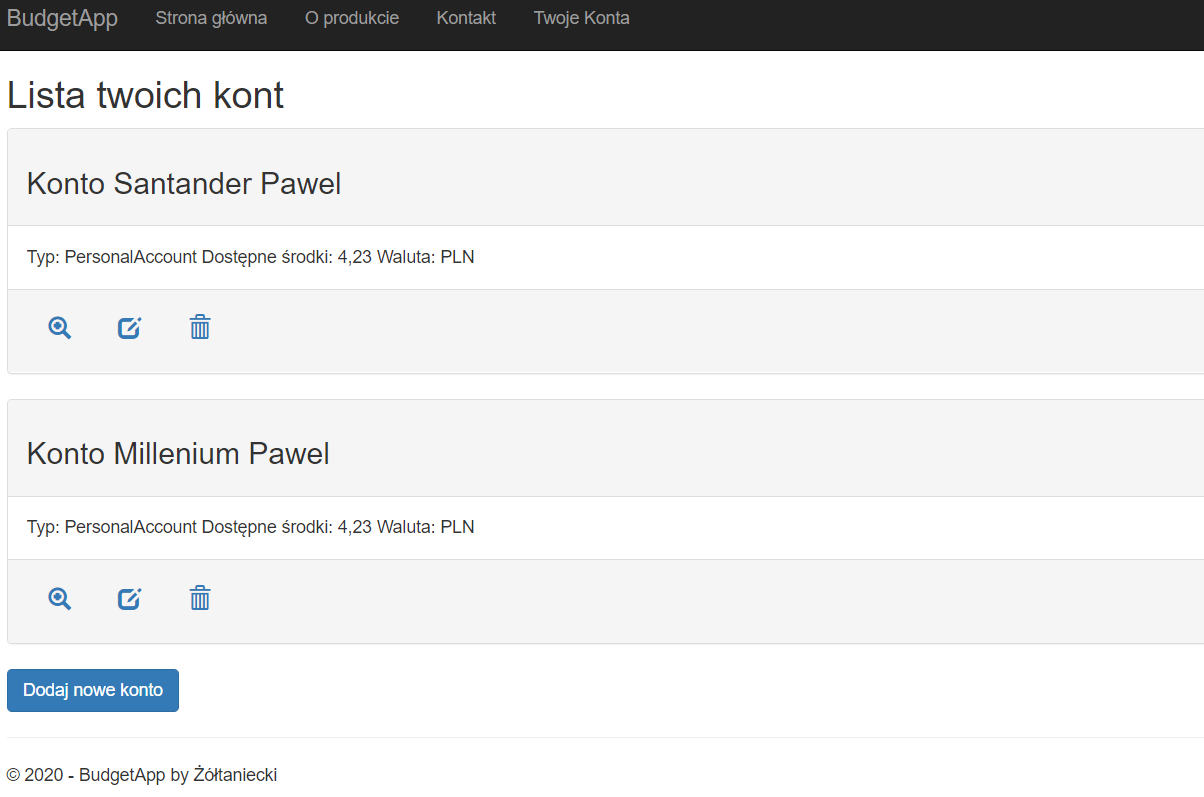
\includegraphics[scale=.35]{rys04/lista-kont.PNG}
	\caption{Widok listy kont użytkownika}
	\label{fig:ss-6}
\end{figure}

Kolejny widok~\ref{fig:ss-1} przedstawia ekran, który pojawia się po naciśnięciu guzika ,,Dodaj nowe konto''. Pojawiają się na nim formularz do wypełnienia przez użytkownika. Aby dodać nowe konto użytkownik musi zatwierdzić dane naciskając guzik ,,Zapisz''.

\begin{figure}[ht]
	\centering
	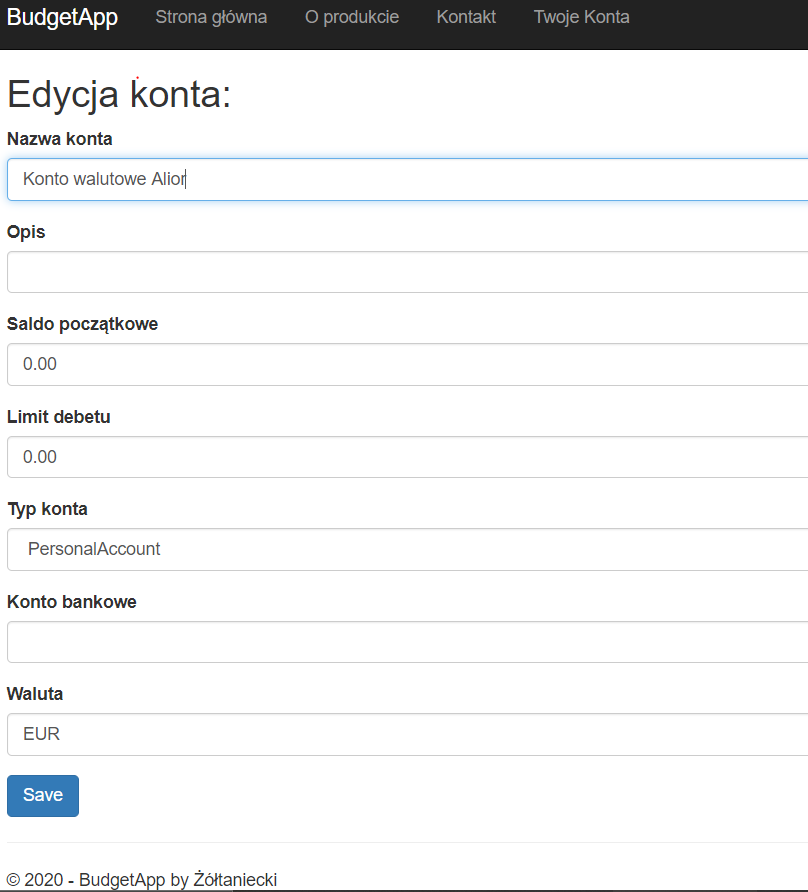
\includegraphics[scale=.35]{rys04/dodaj-konto.PNG}
	\caption{Dodawanie nowego konta}
	\label{fig:ss-1}
\end{figure}

Po dodaniu konta użytkownik znajduje się dalej na tym samym widoku, jednak nie jest to już strona dodania nowego konta, a edycji tego nowostworzonego. Można to zauważyć po zmianie komunikatu z ,,Dodawanie nowego konta'' na ,,Edycja konta: \{nazwa\}''. Pojawia się też jednorazowy komunikat ,,Konto \{nazwa\} zapisano'' -- rysunek~\ref{fig:ss-2}. Znika on po odświeżeniu strony.

\begin{figure}[ht]
	\centering
	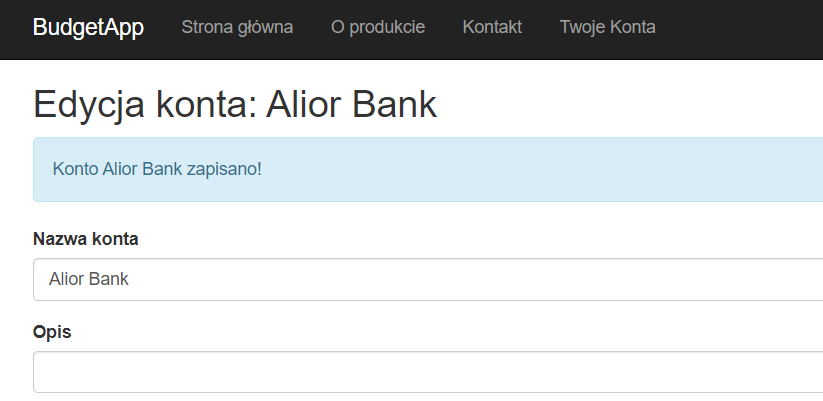
\includegraphics[scale=.35]{rys04/konto-saved.PNG}
	\caption{Edycja stworzonego konta}
	\label{fig:ss-2}
\end{figure}

Z widoku listy kont można także przejść do widoku informacji o koncie -- rysunek~\ref{fig:ss-3}. Na~tym widoku zaprezentowane są informacje o koncie przeznaczone dla użytkownika bez prawa edycji. Guzik powrotu do ekranu listy kont ułatwia sprawną nawigację w aplikacji.

\begin{figure}[ht]
	\centering
	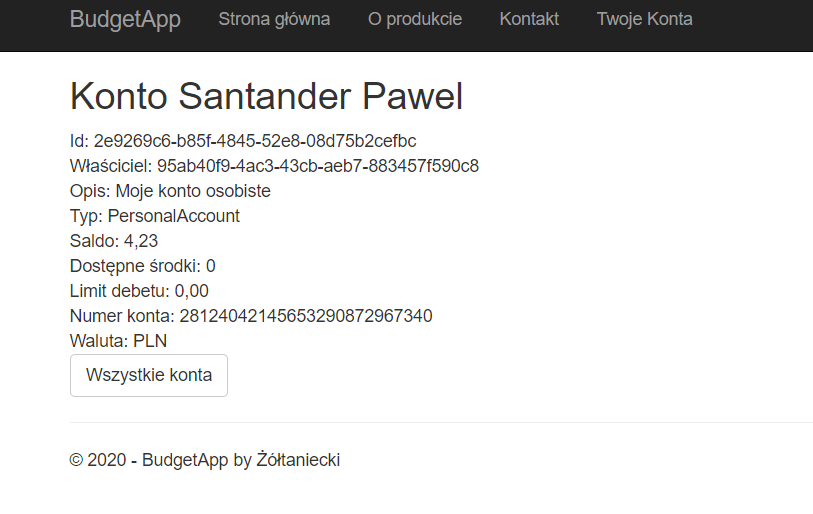
\includegraphics[scale=.35]{rys04/konto-info.PNG}
	\caption{Widok informacji o koncie}
	\label{fig:ss-3}
\end{figure}

Na rysunku~\ref{fig:ss-4} zaprezentowano ekran, pojawiający się po naciśnięciu guzika usuń -- ikonka kosza na śmieci, na stronie z listą kont. Po zatwierdzeniu usunięcia konta użytkownik jest przekierowywany do listy kont. Pojawia się także komunikat o usunięciu strony -- rysunek~\ref{fig:ss-5}.

\begin{figure}[ht]
	\centering
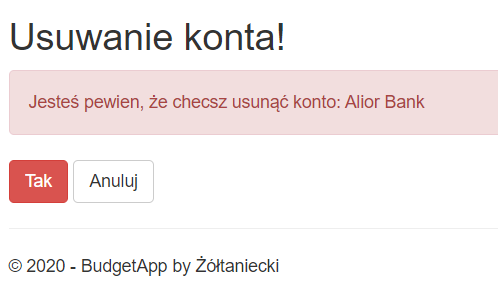
\includegraphics[scale=.35]{rys04/usun-konto.PNG}
	\caption{Usuwanie konta}
	\label{fig:ss-4}
\end{figure}

\begin{figure}[ht]
	\centering
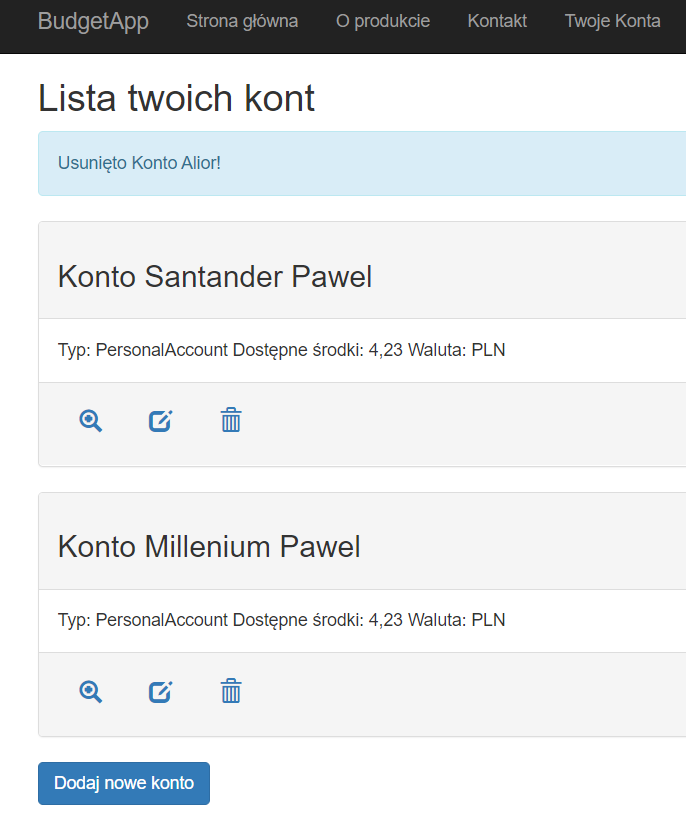
\includegraphics[scale=.35]{rys04/usunieto.PNG}
	\caption{Komunikat o usunięciu konta}
	\label{fig:ss-5}
\end{figure}
\chapter{Uwagi techniczne}% 
\label{chap:testy}
\section{Rysunki}

Rysunki można wstawiać do pracy używając polecenia \verb|\includegraphics|. Zalecane jest, aby pliki z grafikami były umieszczane w katalogach 
odpowiadających numerom rozdziałów czy literom dodatków: \verb|rys01|, \verb|rysA| itd. Sposób wstawiania rysunków do pracy zademonstrowano na przykładze rysunków~\ref{fig:kanji-giri} i \ref{fig:alfabeta}.

\begin{lstlisting}[label=list:includegraphics,caption=Kod źródłowy przykładów wstawiania rysunków do pracy,basicstyle=\footnotesize\ttfamily]
\begin{figure}[ht]
 \centering
  
\includegraphics[width=0.3\linewidth]{rys05/kanji-giri}
 \caption{Dwa znaki kanji - giri}
 \label{fig:kanji-giri}
\end{figure}

\begin{figure}[htb]
 \centering
  \begin{tabular}{@{}ll@{}}
  a) & b) \\
  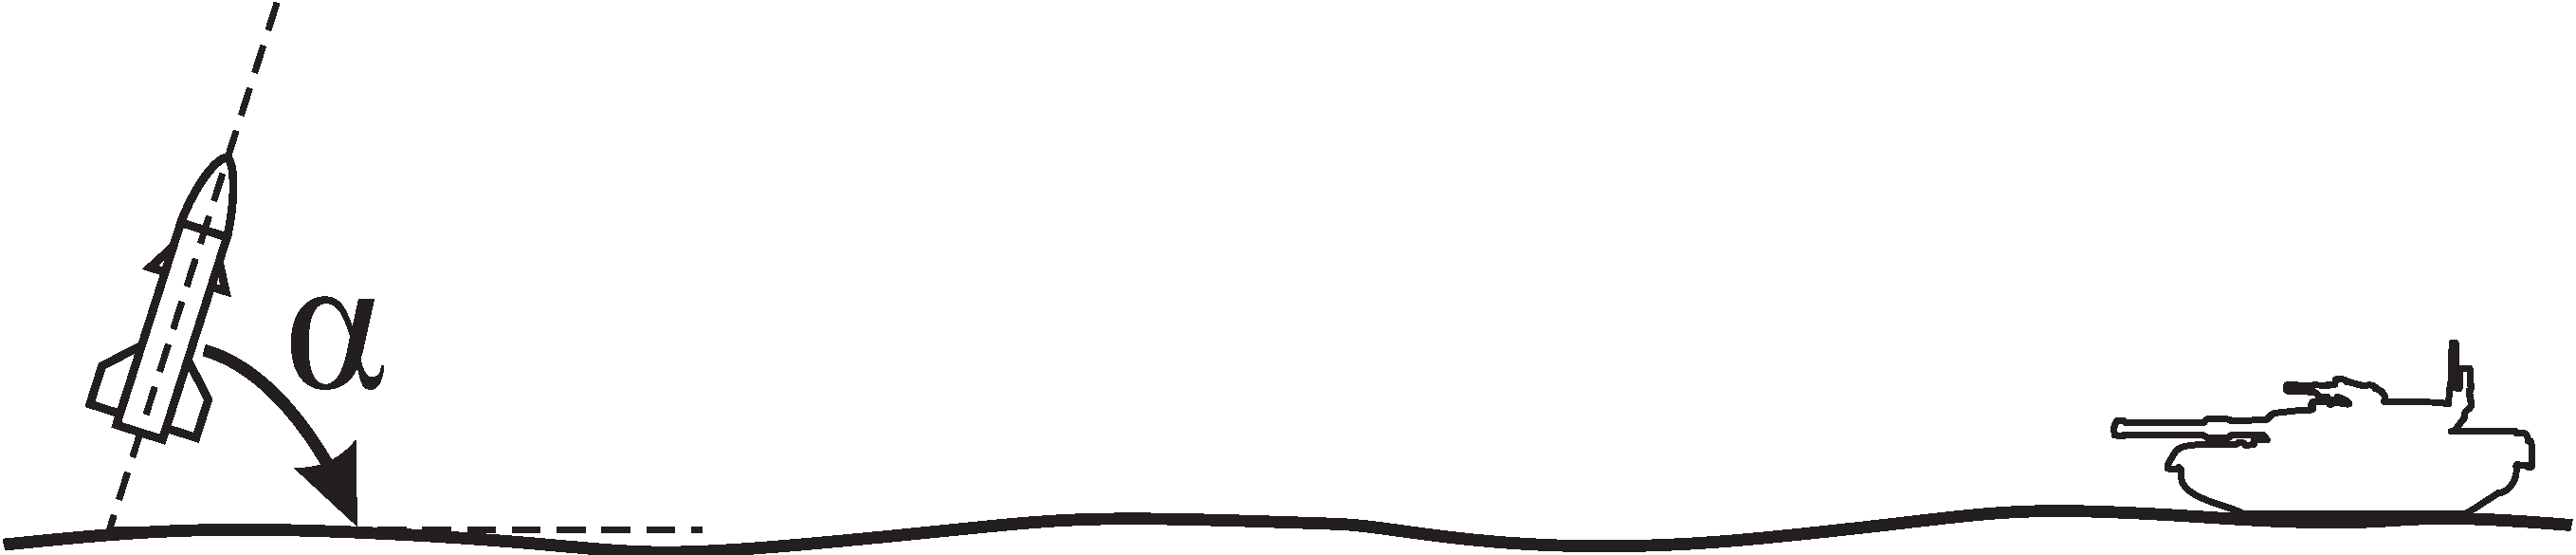
\includegraphics[width=0.475\textwidth]{rys05/alfa1} & 
  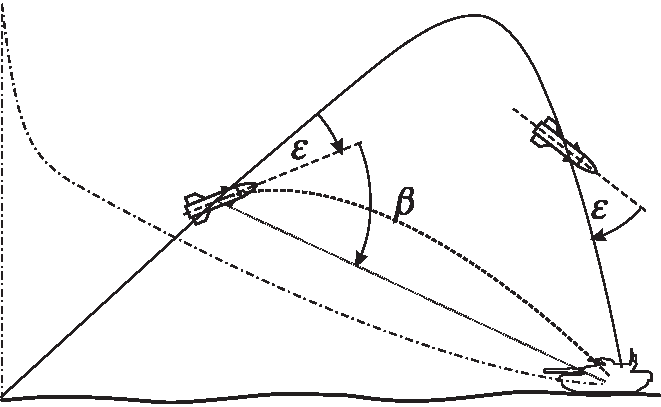
\includegraphics[width=0.475\textwidth]{rys05/beta1}
  \end{tabular}
 \caption{Wyznaczanie trajektorii lotu rakiety: 
 a) trzy podejścia, b) podejście praktyczne}
 \label{fig:alfabeta}
\end{figure}
\end{lstlisting}

\begin{figure}[ht]
	\centering
		
\includegraphics[width=0.3\linewidth]{rys05/kanji-giri}
	\caption{Dwa znaki kanji -- giri}
	\label{fig:kanji-giri}
\end{figure}

\begin{figure}[htb]
  \centering
	\begin{tabular}{@{}ll@{}}
	a) & b) \\
  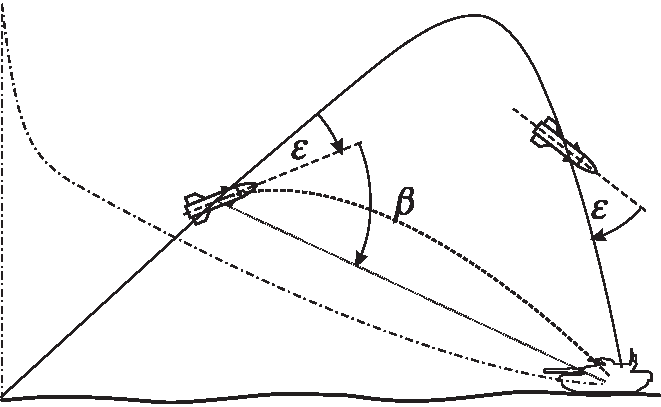
\includegraphics[width=0.475\textwidth]{rys05/beta1} & 
	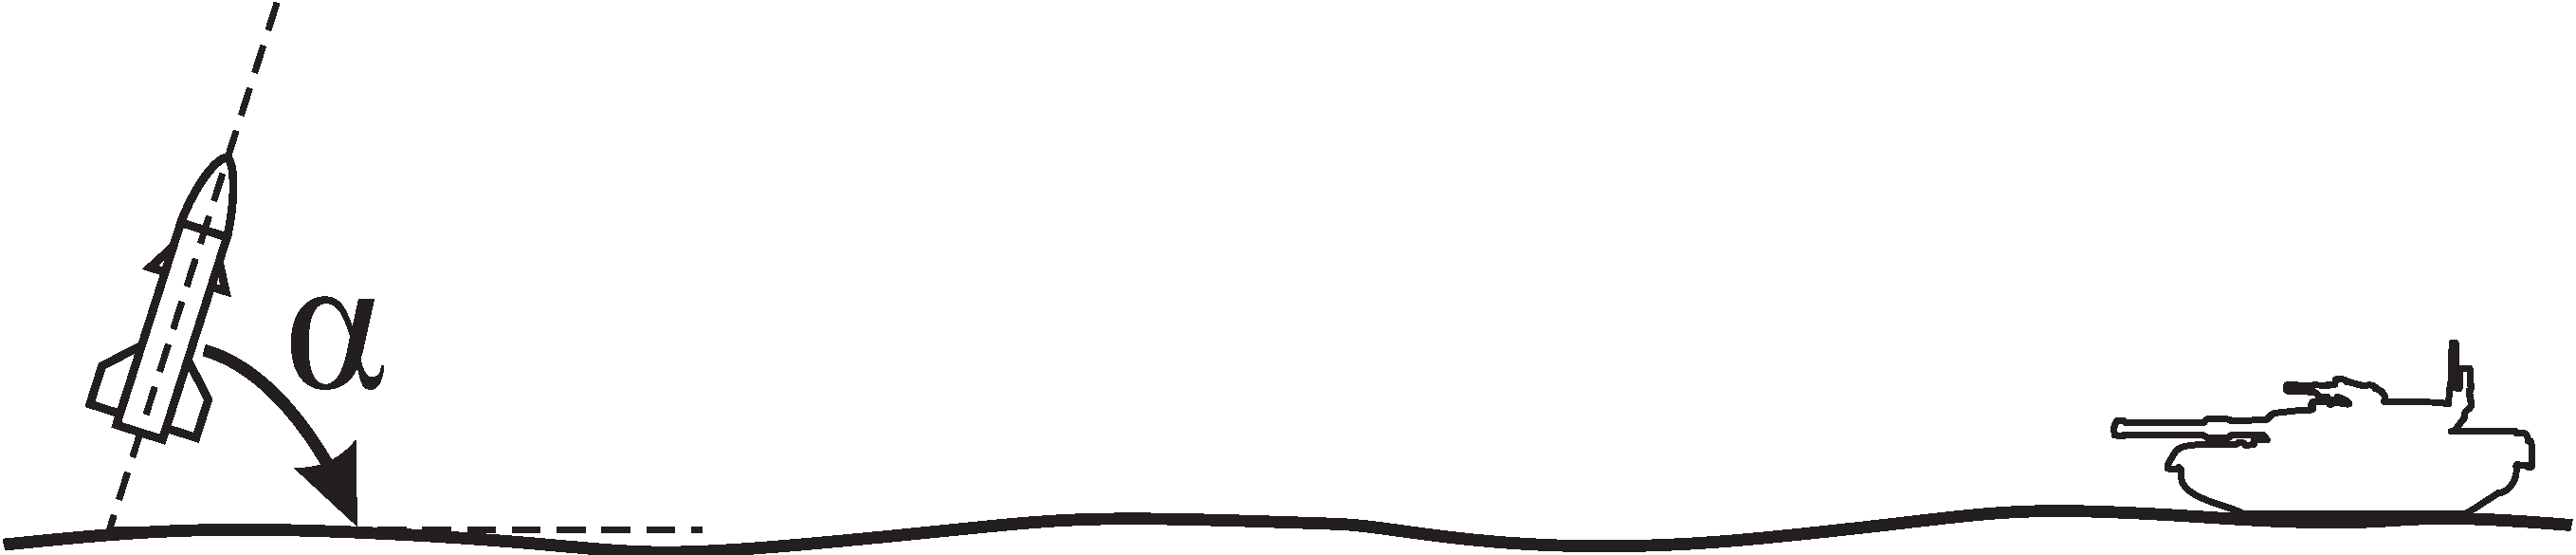
\includegraphics[width=0.475\textwidth]{rys05/alfa1}
	\end{tabular}
  \caption{Wyznaczanie trajektorii lotu rakiety: a) trzy podejścia, b) podejście praktyczne}
  \label{fig:alfabeta}
\end{figure}

Grafiki wektorowe powinny być dostarczone w plikach o formacie pdf. Rozmiar strony w~pliku pdf powinien być troszeczkę większy niż zamieszczona na nim grafika (proszę spojrzeć na przykłady grafik wykorzystanych w niniejszym szablonie). Chodzi o to, aby na rysunku nie pojawiała się niepotrzebna biała przestrzeń. Grafiki rastrowe (głównie zrzuty z ekranu bądź zdjęcia) powinny być dostarczane w plikach o formacie png z~kompresją bezstratną. Zastosowanie kompresji stratnej, jak jpg, wprowadza niepotrzebne artefakty. Podobnie jak w przypadku grafik wektorowych, grafiki rastrowe nie powinny mieć białych marginesów.

Na rysunkach nie powinno stosować się 100\% czarnego wypełnienia, bo robią się plamy przebijające się przez kartkę. Zamiast tego wypełnienie powinno być ok.\ 90\% czerni.

Czcionka na rysunkach nie może być większa od czcionki wiodącej tekstu (jedyny wyjątek to np.\ jakieś nagłówki).
Należy stosować czcionkę kroju Arial, Helvetica bądź tego samego kroju co czcionka dokumentu (\texttt{texgyre-termes}). 

Jeśli na jednym rysunku pojawić się ma kilka grafik, to zamiast stosować \texttt{subfigure} lub inne otoczenia należy wstawić grafiki w tabelę, opisać ją indeksami a) i b), a potem odnieść się do tego w podpisie (rys.~\ref{fig:alfabeta}).
Czasem pomaga w pozycjonowaniu rysunków użycie komendy:
\verb+\vtop{\vskip3ex\hbox{\includegraphics[width=0.475\textwidth]{nazwa}}}+

Na rysunkach nie wolno nadużywać kolorów oraz ozdobników (wiele narzędzi do tworzenia diagramów dostarcza grafikę z cieniowaniem, gradacją kolorów itp.\  co niekoniecznie przekłada się na czytelność rysunku).

Podczas rozbienia zrzutów z ekranu należy zadbać o to, by taki zrzut był czytelny po wydrukowaniu. Czyli aby pojawiające się literki były wystarczająco duże, a przestrzenie bez treści -- relatywnie małe.
Przystępując do robienia zrzutu trzeba odpowiednio wyskalować elementy na ekranie. Na przykład robiąc zrzut z przeglądarki FF najpierw należy wcisnąć CTR--0 (domyślne skalowanie), potem CTR--{}- (zmniejszenie skali o stopień). Potem dobrze jest zawęzić okno przeglądarki tak, by interesująca treść wypełniła je w całości. Jeśli na obserwowanej stronie jest zbyt dużo pustych obszarów, to należy je jakoś zawęzić (sterując wielkością okna przeglądarki lub aktywnymi elementami interfejsu użytkownika). Zrzut bowiem wcale nie musi być odzwierciedleniem 1:1 domyślnego układu obserwowanych elementów. Ważne jest, by na zrzucie z ekranu pokazać interesujący, opisywany fragment i żeby ten fragment był czytelny.
	
Czasem problemem jest tworzenie zrzutów z ekranu, gdy występują na nim dane wrażliwe. Istnieją dwa sposoby na radzenie sobie z tym problemem.
Pierwszy polega na zastąpieniu w~systemie danych danych rzeczywistych danymi testowymi -- wygenerowanymi tylko do celów prezentacji.
Zrzut robi się wtedy na bazie danych testowych.
Drugi polega na wykonaniu zrzutu z~ekranu, na którym pokazano dane rzeczywiste, i następnie zamianie tych danych już w pliku graficznym
za pomocą odpowiedniego edytora (np.~\texttt{gimp}). Czyli oryginalny zrzut z ekranu należy otworzyć w edytorze, a potem
nadpisać oryginalny tekst własnym tekstem. Konieczne jest wtedy dobranie odpowiednich czcionek aby nie było widać
wprowadzonych zmian. 
\begin{quotation}
Uwaga: takie manipulowanie zrzutami jest usprawiedliwione jedynie w przypadku konieczności ochrony danych wrażliwych czy też lepszego pokazania wybranych elementów. Nie może to prowadzić generowania fałszywych rezultatów!!!
\end{quotation}

\section{Wstawianie kodu źródłowego}
Kod źródłowy można wstawiać jako blok tekstu pisany czcionką maszynową. Używa się do tego otoczenie \verb?\lstlisting?. W atrybutach otoczenia można zdefiniować tekst podpisu wstawianego wraz z numerem nad blokiem, etykietę do tworzenia odwołań, sposób formatowania i~inne ustawienia. Zaleca się stosowanie w tym otoczeniu następujących parametrów:
\begin{lstlisting}[basicstyle=\footnotesize\ttfamily]
\begin{lstlisting}[label=list:req1,caption=Initial HTTP Request,
                   basicstyle=\footnotesize\ttfamily]
\end{lstlisting}
Szczególnie przydatne podczas wstawiania większej ilości kodu źródłowego jest zastosowanie parametru \verb+basicstyle=\footnotesize\ttfamily+. Dzięki niemu zmniejsza się czcionka, a~przez to na stronie można zmieścić dłuższe linijki kodu. Użycie tak zdefiniowanego parametru nie jest jednak sztywnym zaleceniem. Wielkość czcionki można dobierać do potrzeb. 
{\belowcaptionskip=-10pt
\begin{lstlisting}[label=list:req1,caption=Initial HTTP Request,
                   basicstyle=\footnotesize\ttfamily]
GET /script/Articles/Latest.aspx HTTP/1.1
Host: www.codeproject.com
Connection: keep-alive
Cache-Control: max-age=0
Accept: text/html,application/xhtml+xml,application/xml
User-Agent: Mozilla/5.0 ...
Accept-Encoding: gzip,deflate,sdch
Accept-Language: en-US...
Accept-Charset: windows-1251,utf-8...
\end{lstlisting}
}
Można też sformatować kod bez stosowania numerowanego podpisu (wtedy nie zamieszcza się \texttt{caption} na liście atrybutów).
\begin{lstlisting}[basicstyle=\footnotesize\ttfamily]
GET /script/Articles/Latest.aspx HTTP/1.1
Host: www.codeproject.com
Connection: keep-alive
Cache-Control: max-age=0
Accept: text/html,application/xhtml+xml,application/xml
User-Agent: Mozilla/5.0 ...
Accept-Encoding: gzip,deflate,sdch
Accept-Language: en-US...
Accept-Charset: windows-1251,utf-8...
\end{lstlisting}

Istnieje możliwość wstawiania kodu źródłowego w bieżącej linijce tekstu. Można to zrobić na kilka sposobów:
\begin{itemize} 
\item korzystając z polecenia \verb?\texttt? ustawiającego czcionkę maszynową, jak w przykładzie \texttt{tutaj} (efekt zastosowania komendy \verb?\texttt{tutaj}?). Problemem jednak mogą okazać się znaki podkreślenia i inne znaki kontrolne.
\item korzystają z otoczenia \verb?\verb? zapewniającego wypisanie kodu czcionką maszynową jak w~przykładzie \verb|tutaj| (efekt zastosowania komendy \verb?\verb|tutaj|?). Problemem jest to, że polecenie \verb?\verb? nie potrafi łamać dłuższego tekstu.
\item korzystając z polecenia \verb?\lstin? umożliwiającego wypisanie kodu czcionką ustawianą w~opcjach jak w przykładzie
\lstset{basicstyle=\ttfamily}\lstinline{tutaj} (efekt komendy \verb+\lstset{basicstyle=\ttfamily}\lstinline{tutaj}+) lub \lstinline[basicstyle=\ttfamily]=tutaj= (efekt komendy \verb+\lstinline[basicstyle=\ttfamily]=tutaj=+).
\end{itemize}

\section{Wykaz literatury oraz cytowania}
\label{sec:literatura}
Cytowania powinny być zamieszczane w tekście z użyciem komendy \verb+\cite{}+. Jej argumentem powinien być klucz cytowanej pozycji (lub lista kluczy  rozdzielonych przecinkiem bez spacji, jeśli takich pozycji w danym miejscu cytuje się więcej) jaki jest używany w bazie danych bibliograficznych (plik \texttt{dokumentacja.bib}). Po kompilacji \texttt{bibtex} i \texttt{pdflatex} w tekście pojawia się właściwy odsyłacz do pozycji w wykazie literatury (ujęty w kwadratowe nawiasy -- zgodnie z~tym, co definiuje styl \texttt{plabbrv.bst}), zaś w samym wykazie (rozdział Literatura) -- zacytowana pozycja. Przykładem cytowania jest: ,,dobrze to opisano w pracach~\cite{JS07,SQL2}'' (gdzie zastosowano komendę \verb?\cite{JS07,SQL2}?).

Co do zawartości rekordów bibliograficznych - style bibtexowe potrafią ,,skracać'' imiona (czyli wstawiać, jeśli taka wola, inicjały zamiast pełnych imion). Niemniej dobrze jest od razu przyjąć jakąś konwencję. Proponuje się, aby w rekordach od razu wstawiane były inicjały zamiast pełnych imion.

Niekiedy tytuły prac zawierają wyrazy z dużymi i małymi literami. Takie tytuły należy brać w podwójne nawiasy klamrowe, aby \texttt{bibtex} nie zamienił ich na postać, w której poza pierwszą literą pozostałe są małe.

Jeśli jakiś cytowany zasób pochodzi z Internetu, to jego rekord w pliku \texttt{bib} powinien wyglądać jak niżej.
\begin{lstlisting}[basicstyle=\footnotesize\ttfamily]
@INPROCEEDINGS{SQL2, 
  title={{A MySQL-based data archiver: preliminary results}}, 
  author={Bickley, M. and Slominski, Ch.},
  booktitle = {{Proceedings of ICALEPCS07}},
	month = oct,
	day = {15--19},
	year={2007}, 
  note={\url{http://www.osti.gov/scitech/servlets/purl/922267} 
	[dostęp dnia 20 czerwca 2015]}
}
\end{lstlisting}
A to inny przykład rekordu danych bibliograficznych:
\begin{lstlisting}[basicstyle=\footnotesize\ttfamily]
@TechReport{JS07,
	author = {Jędrzejczyk, J. and Śródka, B.},
	title  ={Segmentacja obrazów metodą drzew decyzyjnych},
	year = {2007},
	institution = {Politechnika Wrocławska, Wydział Elektroniki}
}
\end{lstlisting}

\section{Indeks rzeczowy}
\label{sec:indeks}
Generowanie indeksu \index{generowanie!-- indeksu} po trosze wygląda jak generowanie wykazu literatury \index{generowanie!-- wykazu literatury}-- wymaga kilku kroków. Podczas pierwszej kompilacji \texttt{pdflatex} generowany jest plik z rozszerzeniem \texttt{*.idx} (zawierający ,,surowy indeks''). Następnie, bazując na tym pliku, generowany jest plik z rozszerzeniem \texttt{*.ind} zawierający sformatowane dane. Ten krok wymaga uruchomienia odpowiedniego narzędzia oraz zastosowania plik z definicją stylu \texttt{Dyplom.ist}. W kroku ostatnim dokonuje się kolejnej kompilacji \texttt{pdflatex} (dzięki niej w wynikowym dokumencie pojawi się Indeks rzeczowy). Domyślnie Indeks rzeczowy zostanie sformatowany w~układzie dwukolumnowym.

Oczywiście aby to wszystko zadziałało w kodzie szablonu należy umieścić odpowiednie komendy definiujące elementy indeksu rzeczowego (\verb?\index?) oraz wstawiające sformatowany Indeks rzeczowy do dokumentu wynikowego (\verb?\printindex?). Więcej informacji o tworzeniu indeksu rzeczowego można znaleźć na stronie \url{https://en.wikibooks.org/wiki/LaTeX/Indexing}. Poniżej przedstawiono przykłady komend użytych w szablonie do zdefiniowania elementów indeksu rzeczowego:
\begin{itemize}
\item \verb?\index{linia komend}? -- pozycji główna.
\item \verb?\index{generowanie!-- indeksu}? -- podpozycja.
\end{itemize}

Generowanie pliku \texttt{*.ind} można inicjować na kilka sposobów:
\begin{itemize}
\item poprzez wydanie odpowiedniego polecenia bezpośrednio w linii komend \index{linia komend}
\begin{lstlisting}[basicstyle=\footnotesize\ttfamily]
makeindex Dyplom.idx -t Dyplom.ilg -o Dyplom.ind -s Dyplom.ist
\end{lstlisting}
\item poprzez odpalenie odpowiedniego narzędzia środowiska. Na przykład w \texttt{TeXnicCenter} definiuje się tzw. \texttt{output profiles}: 
\begin{lstlisting}[basicstyle=\footnotesize\ttfamily]
makeindex "%tm.idx" -t "%tm.ilg" -o "%tm.ind" -s "%tm.ist"
\end{lstlisting}
a samo generowanie pliku \texttt{*.ind} zapewni wybranie pozycji menu \texttt{Build/Makeindex}.
\item korzystając z odpowiednio sparametryzowanych pakietów i komend wewnątrz kompilowanego dokumentu (czyli od razu przy okazji jego kompilacji).
\begin{lstlisting}[basicstyle=\footnotesize\ttfamily]
\DisemulatePackage{imakeidx}
\usepackage[noautomatic]{imakeidx} 
% jeśli chcemy, by indeks by generowany automatycznie programem makeindex:
%\usepackage[makeindex]{imakeidx} 
% a tak ponoć można przekazać opcje do programu generującego indeks:
%\makeindex[options=-s podrecznik -L polish -M lang/polish/utf8] 
%\makeindex[options=-s podrecznik]
\makeindex
\end{lstlisting}

Niestety, \texttt{makeindex} jest narzędziem, które umieszcza część pozycji w grupie \texttt{Symbols}, a~nie w grupach związanych z literkami alfabetu (w związku z czym indeksowany element zaczynający się od polskiej literki trafia do grupy \texttt{Symbols}, jak np.~\verb?\index{Światło}?\index{Światło}. Jeśli chce się zamieszczać w indeksie symbole matematyczne, to dobrze jest to robić jak w następujacym przykładzie: \verb?\index{$asterisk@$\ast$}? \index{$asterisk@$\ast$} czy też \verb?\index{c@$\mathcal{C}$}?\index{c@$\mathcal{C}$}, tj.~dostarczając przy okazji klucz do sortowania.
Lepiej w tym względzie radzą sobie inne narzędzia, jak \texttt{texindy} lub \texttt{xindy} dostępne pod linuxem. Korzystając z nich uzyskuje się grupy polskich literek w indeksie rzeczowym (hasła zaczynające się od polskich literek już nie trafiają do grupy Symbols). Przykład polecenia wydanego z linii komend, w którym wykorzystano \texttt{texindy} zamieszczono poniżej (zakładamy kodowanie plików w UTF8, można dla niniejszego szablonu zmienić na cp1250):
\begin{lstlisting}[basicstyle=\footnotesize\ttfamily]
texindy -L polish -M lang/polish/utf8 Dyplom.idx
\end{lstlisting}

To polecenie wygeneruje \texttt{Dyplom.ind} o zawartości:
\begin{lstlisting}[basicstyle=\footnotesize\ttfamily]
\begin{theindex}
  \providecommand*\lettergroupDefault[1]{}
  \providecommand*\lettergroup[1]{%
      \par\textbf{#1}\par
      \nopagebreak
  }

  \lettergroup{G}
  \item generowanie
    \subitem -- indeksu, 27
    \subitem -- wykazu literatury, 27

  \indexspace

  \lettergroup{L}
  \item linia komend, 27

  \indexspace

  \lettergroup{Ś}
  \item \'Swiat\IeC {\l }o, 28

\end{theindex}
\end{lstlisting}


\end{itemize}


Aby mieć większą kontrolę automatyczne generowanie indeksu zostało w niniejszym szablonie wyłączone (indeks trzeba wygenerować samemu, wydając polecenie \texttt{makeindex} lub zalecane \texttt{texindy}).

\section{Inne uwagi}
Dobrym sposobem na kontrolę błędów występujących podczas kompilacji jest wstawiania linijki \verb?\end{document}? w wybranym miejscu dokumentu. Jest to szczególnie przydatne w przypadkach, gdy błędy te są trudne do zidentyfikowania (gdy wygenerowane przez kompilator numery linii z błędami nie są tymi, w których błędy występują). Wystarczy wtedy przestawić wspomnianą linijkę do kolejnych miejsc, aż znajduję to miejsce, gdzie występuje problem.

Aby osiągnąć apostrofy maszynowe (czyli takie złożone z samych kresek) należy użyć polecenia \verb?"{}jak tutaj{}"? (podwójny apostrof i podwójny apostrof z na wszelki wypadek umieszczonymi nawiasami klamrowymi, nawiasy są potrzebne z tej racji, iż podwójny apostrof przed niektórymi literkami zamienia je na literki z akcentami). W efekcie otrzymamy "{}jak tutaj{}". Jeśli natomiast apostrofy mają być drukarskie (czyli złożone z kropek i kresek), to należy użyć polecenia \verb?,,jak tutaj''? (dwa pojedyncze przecinki i dwa pojedyncze apostrofy). W efekcie otrzymamy ,,jak tutaj''. Można też użyć znaków apostrofów odpowiednio zakodowanych „jak tutaj”, tylko że czasem trudno pisze się takie apostrofy w środowiskach kompilacji projektów latexowych.


Oto sposoby ustawienia odstępów między liniami:
\begin{itemize}
\item używając komendy \verb+\linespread{...}+ (akceptowalne), przy czym atrybutem tej metody jest współczynnik zależny od wielkości
czcionki.  Dla czcionki wiodącej 12pt odstęp półtora linii osiągnie się komendą \verb+\linespread{1.241}+. Dla innych czcionek wiodących wartości tego parametru są jak w poniższym zestawieniu.
\begin{lstlisting}[basicstyle=\footnotesize\ttfamily]
10pt 1.25 dla \onehalfspacing 
     1.667 for \doublespacing, 
		 ponieważ ,,basic ratio'' = 1.2 
		(\normalfont posiada \baselineskip rozmiaru 12pt)
11pt 1.213 dla \onehalfspacing oraz 1.618 dla \doublespacing, 
     ponieważ ,,basic ratio'' = 1.236 
		(\normalfont posiada \baselineskip rozmiaru 13.6pt)
12pt 1.241 dla \onehalfspacing oraz 1.655 dla \doublespacing, 
     ponieważsince ''basic ratio'' is 1.208 
		(\normalfont has a \baselineskip of 14.5pt)
\end{lstlisting}
Kłopot w tym, że raz ustawiony odstęp będzie obowiązywał do wszystkich czcionek (nie działa tu żadem mechanizm zmiany współczynnika w zależności od wielkości czcionki akapitu).

\item używając pakietu \texttt{setspace} (niezalecane). Ponieważ klasa \texttt{memoir} emuluje pakiet \texttt{setspace}, w preambule dokumentu należałoby umieścić:
\begin{lstlisting}[basicstyle=\footnotesize\ttfamily]
\DisemulatePackage{setspace}
\usepackage{setspace}
\end{lstlisting}
a potem można już sterować odstęp komendami:
\begin{lstlisting}[basicstyle=\footnotesize\ttfamily]
\singlespacing
\onehalfspacing
\doubelspacing
\end{lstlisting}
Ten sposób pozwala na korzystanie z mechanizmu automatycznej zmiany odległości linii w~zależności od wielkości czcionki danego akapitu.
\item korzystając bezpośrednio z komend dostarczonych w klasie \texttt{memoir} (zalecane):
\begin{lstlisting}[basicstyle=\footnotesize\ttfamily]
\SingleSpacing
\OnehalfSpacing
\DoubleSpacing
\end{lstlisting}
Ten sposób również pozwala na korzystanie z mechanizmu automatycznej zmiany odległości linii w zależności od wielkości czcionki danego akapitu.
\end{itemize}

Na koniec jeszcze uwaga o rozmiarze pliku wynikowego. Otóż \texttt{pdflatex} generuje pliki \texttt{pdf}, które zazwyczaj mogłyby być nieco lepiej
skompresowane. Do lepszego skompresowania tych plików można użyć programu \texttt{ghostscript}. Wystarczy w tym celu wydać komendę (pod windowsami):
\begin{lstlisting}[basicstyle=\footnotesize\ttfamily]
gswin64 -sDEVICE=pdfwrite -dCompatibilityLevel=1.4 -dNOPAUSE -dQUIET -dBATCH 
-sOutputFile=Dyplom-compressed.pdf Dyplom.pdf
\end{lstlisting}

\chapter{Podsumowanie}
\label{chap:podsumowanie}
Celem pracy było zbudowanie systemu do zarządzania domowym budżetem o minimalnej wartości użytkowej. System miał umożliwiać użytkownikowi sprawne zarządzanie wydatkami i~przychodami, w szczególności z podziałem na wiele kont bankowych. W jego skład miały wchodzić dwie aplikacje webowe: kliencka -- dostarczająca interfejs użytkownika w przeglądarce oraz API -- gwarantująca szybkie i poprawne, z biznesowego punktu widzenia, przetwarzanie żądań aplikacji klienckiej. Obie te aplikacje zostały stworzone i są gotowe do działania w środowisku produkcyjnym oraz dalszego rozwoju.

Funkcjonalności dotyczące zarządzania kontami pieniężnymi i środkami finansowymi w ramach rodziny, a zdefiniowane w zakresie pracy, zostały szczegółowo przeanalizowane i opisane z wykorzystaniem technik inżynierii oprogramowania oraz języka UML. Autor szczegółowo opisał ich przypadki użycia, dzieląc system na cztery mniejsze podsystemy.

Funkcjonalności obsługi konta bankowego i manipulowania jego środkami finansowymi zostały zaimplementowane dla indywidualnego użytkownika. Użytkownik może dodawać konta, a także operacje finansowe po zalogowaniu się do systemu.

Funkcjonalności dotyczące obsługi całej rodziny zostały zaprojektowane i opisane. Jednak zgodnie z zakresem pracy nie zostały zaimplementowane.

Niestety aplikacja kliencka od strony graficznej nie została wykonana w sposób zadowalający. Spełnia ona swoje wymagania funkcjonalne, jednak jej szata graficzna korzysta z domyślnego ostylowania, zapewnionego przez środowisko programistyczne Visual Studio.

Przy okazji tworzenia pracy autor zapoznał się z wieloma wzorcami projektowymi takimi jak mediator, \emph{Command Query Responsibility Segregation} cz \emph{Model–view–viewmodel}. Autor zgłębił także dobre praktyki tworzenia oprogramowania, a w szczególności interfejsu programistycznego API. Autor wykorzystał zdobytą wiedzę do stworzenia elastycznego oprogramowania gotowego do dalszego rozwoju w profesjonalnym środowisku deweloperskim. Oprogramowanie jest także stworzone z wykorzystaniem najlepszych praktyk sztuki zawodowej, które ułatwiają utrzymanie aplikacji.

Autor przetestował także aplikację kliencką oraz API, tak aby zapewnić najwyższą jakość dostarczanego oprogramowania i świadczonych przez nie usług. Testy zostały wykonany w~sposób rzetelny i dokładny. Potwierdziły dobrą jakość stworzonego oprogramowania i gotowość używania go w środowisku produkcyjnym.

Aplikacja po zaimplementowaniu reszty funkcjonalności, spełniać będzie założenia postawione przez autora i stanie się uniwersalnym narzędziem do zarządzania domowym budżetem, ze szczególną kontrolą administratora rodziny.

W przyszłości aplikacja może zostać poszerzona o funkcje związane z generowaniem wydatków na podstawie zdjęć paragonów, a także tworzenie ich kopii zapasowej w celu zarządzania gwarancjami produktów. W aplikacji mogą również znaleźć się funkcje umożliwiające przechowywanie kart lojalnościowych, bonów i innych dokumentów sprzedażowych.


%\bibliographystyle{plalpha}
\bibliographystyle{plabbrv}

%UWAGA: bibliotekę referencji należy przygotować samemu. Dobrym do tego narzędziem jest JabRef.
%       Nazwę przygotowanej biblioteki wpisuje się poniżej bez rozszerzenia 
%       (w tym przypadku jest to "dokumentacja.bib")
\bibliography{dokumentacja}
\appendix
\chapter{Instrukcja uruchomienia aplikacji}

Aby uruchomić aplikację w lokalnym środowisku deweloperskim należy:

\begin{itemize}
\item Zainstalować środowisko programistyczne Visual Studio 2017 lub 2019. 
\item Uruchomić w programie Visual Studio solucję BudgetApplicationAPI.
\item Prawym guzikiem nacisnąć na projekt \texttt{Zoltaniecki.IDP} i wybrać opcję \texttt{Set as StartUp Project}
\item Kombinacją klawiszy \texttt{ctrl + F5} lub wybierając z menu: \texttt{Debug > Start without Debugging} uruchomić serwer dostawcy tożsamości.
\item Prawym guzikiem nacisnąć na projekt \texttt{BudgetApplication.API} i wybrać opcję \texttt{Set as StartUp Project}
\item Kombinacją klawiszy \texttt{ctrl + F5} lub wybierając z menu: \texttt{Debug > Start without Debugging} uruchomić serwer API.
\item Uruchomić drugi raz Visual Studio i otworzyć w nim solucję BudgetApplicationClient.
\item Prawym guzikiem nacisnąć na projekt \texttt{BudgetApplication.Client} i wybrać opcję \texttt{Set as StartUp Project}
\item Kombinacją klawiszy \texttt{ctrl + F5} lub wybierając z menu: \texttt{Debug > Start without Debugging} uruchomić serwer aplikacji klienckiej.
\item Login: Frank, hasło: password
\end{itemize}


\chapter{Opis załączonej płyty DVD}
Na załączonej płycie DVD znajduje się plik tekstowy z treścią pracy inżynierskiej w formacie \texttt{.pdf}, a także repozytorium kodu źródłowego wykonanych aplikacji. Poniżej przedstawiono strukturę głównych folderów znajdujących się na płycie.
{\small
\begin{verbatim}
D:.
├───Dokument
│   └───praca-inzynierska.pdf
└───repo
    └───BudgetApp
        └───src
            ├───API
            │   ├───BudgetApplication.API
            │   ├───BudgetApplication.Domain
            │   ├───BudgetApplication.Infrastructure
            │   └───BudgetApplication.QueryInfrastructure
            └───Client
                ├───BudgetApplication.Client
                └───BudgetApplication.Client.Core
\end{verbatim}
}

\chapterstyle{noNumbered}
\phantomsection % sets an anchor
\addcontentsline{toc}{chapter}{Indeks rzeczowy}
\printindex

\end{document}
